\documentclass{article}
\usepackage{amsmath,amssymb,amsthm,kotex,mdframed,paralist}

\newcounter{num}
\newcommand{\defi}[1]
{\bigskip\noindent\refstepcounter{num}\textbf{정의 \arabic{num}) #1}\par}
\newcommand{\theo}[1]
{\bigskip\noindent\refstepcounter{num}\textbf{정리 \arabic{num}) #1}\par}
\newcommand{\exam}[1]
{\bigskip\noindent\refstepcounter{num}\textbf{예시 \arabic{num}) #1}\par}
\newcommand{\prob}[1]
{\bigskip\noindent\refstepcounter{num}\textbf{문제 \arabic{num}) #1}\par}


\renewcommand{\proofname}{증명)}
\newcommand{\mo}[1]{\ensuremath{\:(\text{mod}\:\:#1)}}

%%%
\begin{document}

\title{영석 : 03 중간고사(1학년 1학기) 대비 개념 요약}
\author{}
\date{\today}
\maketitle
\tableofcontents
\newpage

%%%
\section{다항식의 연산}
%%
\subsection{다항식}
%
\defi{다항식}
\(2x^2+3x-1\), \(x+1\), \(x^3\), \(x^2+2xy+2y^2\) 등의 형태의 식을 \textbf{다항식}이라고 한다.
특히 항의 개수가 한 개인 다항식을 \textbf{단항식}이라고 한다.
예를 들어 \(x^3\)는 단항식이지만 \(2x^2+3x-1\), \(x+1\)는 단항식이 아니다.

다항식
\[2x^2+3x-1\tag{1}\]
에서 \(2x^2\), \(3x\), \(-1\)를 \textbf{항}이라고 한다.

각 항의 문자 앞에 붙는 숫자를 \textbf{계수}라고 한다.
\(2x^2\)의 계수는 \(2\)이고 \(3x\)의 계수는 \(3\)이다.
숫자로만 되어있는 항을 \textbf{상수항}이라고 한다.
각 항들에 대해 문자가 곱해진 개수를 \textbf{차수}라고 한다.
\(2x^2\)의 차수는 2차이고, \(3x\)의 차수는 1차이다.
다항식의 차수는 각 항들 중 가장 높은 항의 차수를 말한다.
\(2x^2+3x-1\)의 차수는 2차이다.

(1)에서처럼 다항식을 차수가 높은 항부터 나열하는 방식을 \textbf{내림차순}이라고 한다.
반대로 (2)와 같이 차수가 낮은 항부터 나열하는 방식을 \textbf{오름차순}이라고 한다.
\[-1+3x+2x^2\tag{2}\]

%%
\subsection{다항식의 덧셈과 뺄셈}
다항식을 더하고 뺄 때에는 동류항을 묶어서 계산하면 된다.
실수와 마찬가지로 덧셈과 곱셈에 대해 교환법칙과 결합법칙, 분배법칙이 성립한다.

%
\theo{다항식의 연산법칙}
\(A\), \(B\), \(C\)가 다항식이면
\begin{align*}
&A+B=B+A,\quad AB=BA 				\tag{교환법칙}\\
&(A+B)+C=A+(B+C),\quad (AB)C=A(BC)	\tag{결합법칙}\\
&A(B+C)=AB+AC						\tag{분배법칙}
\end{align*}
이 성립한다.

%
\exam{}
예를 들어 \(2x^2+3x+2\)와 \(x^2-2x+1\)을 더하면
\begin{align*}
(2x^2+3x+2)+(x^2-2x+1)
&=(2x^2+x^2)+(3x-2x)+(2+1)\\
&=3x^2+x+3
\end{align*}
이다.

또 \(x^2+y^2\)과 \(2x^2+2xy-4y^2\)을 빼면
\begin{align*}
(x^2+y^2)-(2x^2+2xy-4y^2)
&=(x^2-2x^2)-2xy+(y^2-(-4y^2))\\
&=-x^2-2xy+5y^2
\end{align*}
이다.


%%
\subsection{다항식의 곱셈}
다항식을 곱할 때에는 분배법칙을 잘 적용해 곱하면 된다.
또한 다음 공식들을 사용할 수 있다.

%
\theo{곱셈공식}\label{mul.formula}
\begin{enumerate}[(1)]
\item
\((a+b)^2=a^2+2ab+b^2\)
\item
\((a-b)^2=a^2-2ab+b^2\)
\item
\((a-b)(a+b)=a^2-b^2\)
\item
\((a+b+c)^2=a^2+b^2+c^2+2(ab+bc+ca)\)
\item
\((a+b)^3=a^3+3a^2b+3ab^2+b^3\)
\item
\((a-b)^3=a^3-3a^2b+3ab^2-b^3\)
\item
\((a+b)(a^2-ab+b^2)=a^3+b^3\)
\item
\((a-b)(a^2+ab+b^2)=a^3-b^3\)
\end{enumerate}

%
\exam{}
(1) 예를 들어
\((2x+1)^2\)을 전개하려면 정리 \ref{mul.formula}의 (1)에 \(a=2x\), \(b=1\)을 대입하여
\[(2x+1)^2=(2x)^2+2\times(2x)\times1+1^2=4x^2+4x+1\]
을 얻을 수 있다.

(2) \((x-2)^3\)을 전개하려면 정리 \ref{mul.formula}의 (6)에 \(a=x\), \(b=2\)를 대입하여
\[(x-2)^3=x^3-3\times x^2\times2+3\times x\times2^2-2^3=x^3-6x^2+12x-27\]
을 얻을 수 있다.

%%
\subsection{다항식의 나눗셈}
\exam{}\label{div}
만약 \(2x^3+7x^2+3\)을 \(x^2+2x+2\)로 나누려면 다음과 같은 계산을 한다.
\begin{figure}[h]
\center
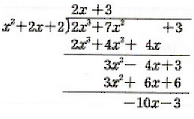
\includegraphics{01_04_division}
\end{figure}

따라서 몫이 \(2x+3\)이고 나머지가 \(-10x-3\)이다.
이 나눗셈 결과를 다음과 같이 표현한다.
\[2x^3+7x+3=(x^2+2x+2)(2x+3)+(-10x-3)\]
이다.

일반적으로 \(A\)를 \(B\)로 나눈 몫이 \(Q\)이고 나머지가 \(R\)이면
\[A=BQ+R\]
이라고 쓴다.
여기서 \(A\), \(B\), \(Q\), \(R\)은 모두 다항식이며, 각각 \textbf{피제수}, \textbf{제수}, \textbf{몫}, \textbf{나머지}라고 부른다.
또 \(R\)의 차수는 \(B\)보다 항상 작다.
위의 예에서도 나머지(=\(-10x-3\))의 차수가 제수(=\(x^2+2x+2\))의 차수보다 낮다는 것을 확인할 수 있다.

%%%%
\section{항등식과 나머지 정리}

%%
\subsection{항등식}
%
\defi{항등식}
\textbf{항등식}이란, 문자에 어떤 값을 대입해도 항상 성립하는 등식을 말한다.
항등식에서 아직 정해지지 않은 경우의 계수를 \textbf{미정계수}라고 부른다.
항등식이 아닌 등식을 \textbf{방정식}이라고 한다.

%
\exam{}
예를 들어 \(x^2+2x=x^2+2x\)는 \(x\)에 어떤 값을 대입하더라도 성립하기 때문에 항등식이다.
마찬가지로 \(2x=2x\), \(x+1-x=1\) 등도 항등식이다.
하지만 \(2x+2=0\)은 \(x=-1\)일 때는 성립하지만 \(x\neq-1\)일 때에는 성립하지 않으므로 항등식이 아니고 방정식이다.

%
\theo{항등식의 성질}\label{prop._of_id.eq.}
\begin{enumerate}[(1)]
\item
\(ax+b=0\)이 항등식이면 \(a=0\), \(b=0\)이다.
\item
\(ax^2+bx+c=0\)이 항등식이면 \(a=0\), \(b=0\), \(c=0\)이다.
\item
\(ax+by+c=0\)이 항등식이면 \(a=0\), \(b=0\), \(c=0\)이다.
\item
\(ax+b=a'x+b'\)가 항등식이면 \(a=a'\), \(b=b'\)이다.
\item
\(ax^2+bx+c=a'x^2+b'x+c'\)이 항등식이면 \(a=a'\), \(b=b'\), \(c=c'\)이다.
\item
\(ax+by+c=a'x+b'y+c'\)이 항등식이면 \(a=a'\), \(b=b'\), \(c=c'\)이다.
\end{enumerate}
(1)--(6)의 역도 성립한다.

\begin{proof}
(1)과 (4)만 증명하겠다.

(1) \(ax+b=0\)가 항등식이라고 하자.
\(x\)에 대한 항등식이므로 \(x\)에 어떤 값을 대입하더라도 성립한다.
\(x=0\)을 대입하면 \(a=0\)을 얻는다.
이제 원래 식은 \(b=0\)이 되었고 이는 성립해야 한다.
따라서 \(a=0\)이고 \(b=0\)이다.

반대로 \(a=0\), \(b=0\)이라고 하자.
그러면 본 식은
\(0=0\)이 되어 항등식이다.

(4) \(ax+b=a'x+b'\)가 항등식이라고 하자.
그러면 모든 항을 좌변으로 이항한 식인
\[(a-a')x+(b-b')=0\]
은 항등식이다.
(1)에 의해 \(a-a'=0\)이고 \(b-b'=0\)이다.

반대로 \(a=a'\), \(b=b'\)이라고 하자.
그러면 본 식은 \(ax+b=ax+b\)가 되어 \(x\)에 어떤 값을 넣더라도 항상 성립한다.
따라서 항등식이다.


\end{proof}

%%
%\exam{}
%예를 들어 \(2x+3=2x+3\)은 \(a=2\), \(b=3\), \(a'=2\), \(b'=3\)이라서 \(a=a'\), \(b=b'\)이므로 정리 \ref{prop.of.id.eq}의 (4)에 의해 항등식이다.
%또 \(x+y+1=2x+y+1\)은 \(a=1\), \(b=1\), \(c=1\), \(a'=2\), \(b'=1\), \(c'=1\)이라서 \(a\neq a'\)이므로 정리 \ref{prop.of.id.eq}의 (6)에 의해 항등식이 아니다.
%\(x+3=0\)은 정리 \ref{prop.of.id.eq}의 (1)에서 \(a=1\), \(b=3\)이므로 항등식이 아니다.
%정리 \ref{prop.of.id.eq}의 (4)로 생각하여 \(a=1\), \(b=3\), \(a'=0\), \(b'=0\)이고 \(a\neq a'\)이고 \(b\neq b'\)이므로 항등식이 아니라고 말할 수도 있다.

%
\exam{}\label{id.eq.ex.01}
(1)
항등식
\[(a-2)x+(b+3)=0\]
에서 미정계수 \(a\), \(b\)를 구해보자.
정리 \ref{prop._of_id.eq.}의 (1)에 의해 \(a-2=0\), \(b+3=0\)이다.
따라서 \(a=2\), \(b=-3\)이다.

(2)
항등식
\[(a+1)x-by+(c+1)=0\]
에서 미정계수 \(a\), \(b\), \(c\)를 구해보자.
정리 \ref{prop._of_id.eq.}의 (3)에 의해 \(a+1=0\), \(-b=0\), \(c+1=0\)이다.
따라서 \(a=-1\), \(b=0\), \(c=-1\)이다.

(3)
항등식 
\[-2x^2-ax+3=bx^2+5x-c+1\]
에서 미정계수 \(a\), \(b\), \(c\)를 구해보자.
정리 \ref{prop._of_id.eq.}의 (5)에 의해 \(-2=b\), \(-a=5\), \(3=-c+1\)이다.
따라서 \(b=-2\), \(a=-5\), \(c=-2\)이다.

%
\exam{}\label{id.eq.ex.02}
(1)
항등식
\[a(x+1)+b(x-1)=3x+1\]
의 미정계수 \(a\), \(b\)를 구할 때에는 좌변을 전개하여
\[(a+b)x+(a-b)=3x+1\]
를 얻고, 정리 \ref{prop._of_id.eq.}의 (4)를 이용해 연립방정식
\begin{gather*}
a+b=3\\
a-b=1
\end{gather*}
을 풀어 \(a=2\), \(b=1\)이라는 결과를 얻을 수도 있으나 이 경우에는 다른 방법을 사용하는 것이 더 간편할 수 있다.

원래 식인
\[a(x+1)+b(x-1)=3x+1\]
에 \(x=1\)을 넣으면 \(2a=4\)를 얻고 \(x=-1\)을 넣으면 \(-2b=-2\)를 얻으므로 한번에 \(a=2\), \(b=1\)을 얻을 수 있기 때문이다.

(2)
마찬가지로 항등식
\[ax(x+1)+bx(x-1)+c(x+1)(x-1)=2x^2-3x+3\]
의 미정계수 \(a\), \(b\), \(c\)를 구할 때에도 \(x\)에 값들을 대입하는 방법이 더 효율적이다.
\(x=0\)을 대입하면 \(-c=3\)를 얻고, \(x=1\)을 대입하면 \(2a=2\)를 얻으며, \(x=-1\)를 대입하면 \(2b=8\)을 얻는다.
따라서 \(c=-3\), \(a=1\), \(b=4\)이다.

%
\defi{}
항등식에서 미정계수를 구할 때에
예시 \ref{id.eq.ex.01}에서 사용한 방법을 \textbf{계수비교법}, 
예시 \ref{id.eq.ex.02}에서 사용한 방법을 \textbf{수치대입법}이라고 한다.

%
\theo{}\label{div.theo.}
다항식 \(f(x)\)를 다항식 \(g(x)\)로 나누었을 때의 몫을 \(Q(x)\), 나머지를 \(R(x)\)라고 하면,
\[f(x)=g(x)Q(x)+R(x)\]
가 성립하며 이 때의 등식은 항등식이다.

%
\defi{}
정리 \ref{div.theo.}에서 \(R(x)=0\)이면 \(f(x)\)가 \(g(x)\)로 \textbf{나누어 떨어진다}고 말한다.
혹은 \(g(x)\)가 \(f(x)\)의 \textbf{인수}라고 말한다.

%%
\subsection{나머지 정리와 인수정리}

%
\theo{나머지 정리}\label{remainder}
다항식 \(f(x)\)를 \(x-\alpha\)로 나눈 나머지는 \(f(\alpha)\)이다.
\begin{proof}
\(f(x)\)를 \(x-\alpha\)로 나누었을 때의 몫을 \(Q(x)\)라고 하고 나머지를 \(R(x)\)라고 하자.
\(R(x)\)의 차수는 피제수인 \(x-\alpha\)의 차수보다 작으므로, \(R(x)\)는 상수항이다.
따라서 \(R(x)=R\)이라고 쓰자.
그러면
\[f(x)=(x-\alpha)Q(x)+R\]
은 항등식이다.
이 항등식에 \(x=\alpha\)를 대입하면 \(f(\alpha)=R\)을 얻는다.
따라서 이 나눗셈의 나머지는 \(f(\alpha)\)이다.
\end{proof}

%
\exam{}
예시 \ref{div}에서 이용한 방법을 사용해 \(f(x)=x^2+1\)을 \(x+1\)로 나누면 \(x^2+1=(x+1)(x-1)+2\)이다.
따라서 \(f(x)\)를 \(x+1\)로 나누었을 때의 나머지는 \(2\)이다.
정리 \ref{remainder}를 사용해 \(f(x)\)를 \(x+1\)로 나눈 나머지를 계산하려면 \(x+1=x-(-1)\)이므로 \(\alpha=-1\)이고, 따라서 나머지는 \(f(-1)\)이어야 한다.
실제로 \(f(-1)=(-1)^2+1=2\)이다.

마찬가지로 \(g(x)=x^2+2x+2\)를 \(x-1\)로 나눈 나머지는 \(g(1)=1^2+2\cdot1+2=5\)이고 \(h(x)=-x^2+3x+1\)을 \(x-2\)로 나눈 나머지는 \(h(2)=-2^2+3\cdot2+1=3\)이다.

%
\theo{인수정리}
다항식 \(f(x)\)가 \(x-\alpha\)로 나누어떨어지면 \(f(\alpha)=0\)이고, \(f(\alpha)=0\)이면 \(f(x)\)가 \(x-\alpha\)로 나누어떨어진다.
\begin{proof}
\(f(x)\)를 \(x-\alpha\)로 나누었을 때의 나머지를 \(R\)이라고 하면
나머지 정리에 의해 \(R=f(\alpha)\)이다.
\(f(x)\)가 \(x-\alpha\)로 나누어떨어지면 \(R=0\)이다.
따라서 \(f(\alpha)=0\)이다.
반대로 \(f(\alpha)=0\)이면 \(R=0\)이다.
따라서 \(f(x)\)는 \(x-\alpha\)로 나누어떨어진다.
\end{proof}

%
\exam{}\label{factor.theo.}
\(f(x)=x^3-3x+2\)라고 하자.
\(x=1\)을 대입하면 \(f(1)=1^3-3\cdot1+2=0\)이므로 \(x-1\)은 \(f(x)\)의 인수이다.
\(x=2\)를 대입하면 \(f(2)=2^3-3\cdot2+2\neq0\)이므로 \(x-2\)는 \(f(x)\)의 인수가 아니다.

%
\exam{}


%%
\subsection{조립제법}
다항식의 나눗셈에서 제수가 일차식이면 \textbf{조립제법}을 활용하면 쉽게 몫과 나머지를 구할 수 있다.
다음은 \(-x^4+3x^3+6x^2-6x-5\)를 \(x+2\)로 나누는 과정을 나타낸 것이다.
\begin{figure*}[h]
\center
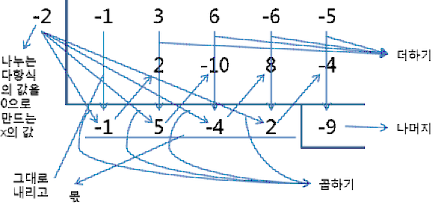
\includegraphics[width=0.65\textwidth]{02_03_synthetic_division}
\end{figure*}

이 나눗셈에서 몫은 \(-x^3+5x^2-4x+2\)이고, 나머지는 \(-9\)이다.
따라서
\[-x^4+3x^3+6x^2-6x-5=(x+2)(-x^3+5x^2-4x+2)-9\]
이다.

%%%
\section{인수분해}

%
\defi{전개와 인수분해}
\((x+1)(x+2)\)를 전개하면 \(x^2+3x+2\)이고 \(x^2+3x+2\)를 인수분해하면 \((x+1)(x+2)\)가 된다.
이처럼 \textbf{전개}란 곱셈으로 묶여있는 다항식을 푸는 과정을 뜻하며 \textbf{인수분해}란 풀어져 있는 다항식을 곱셈으로 묶는 과정을 뜻한다.

%
\theo{인수분해공식}\label{fac.formula}
정리 \ref{mul.formula}의 곱셈공식의 좌변과 우변을 바꿔 다음과 같은 인수분해 공식들을 얻는다.
\begin{enumerate}[(1)]
\item
\(a^2+2ab+b^2=(a+b)^2\)
\item
\(a^2-2ab+b^2=(a-b)^2\)
\item
\(a^2-b^2=(a-b)(a+b)\)
\item
\(a^2+b^2+c^2+2(ab+bc+ca)=(a+b+c)^2\)
\item
\(a^3+3a^2b+3ab^2+b^3=(a+b)^3\)
\item
\(a^3-3a^2b+3ab^2-b^3=(a-b)^3\)
\item
\(a^3+b^3=(a+b)(a^2-ab+b^2)\)
\item
\(a^3-b^3=(a-b)(a^2+ab+b^2)\)
\end{enumerate}

%
\exam{}
(1)
\[x^2-2x+1\]
를 인수분해해보자.
정리 \ref{fac.formula}의 (2)에 \(a=x\), \(b=1\)를 넣으면
\[x^2-2x+1=(x-1)^2\]
를 얻는다.
따라서 \(x^2-2x+1\)를 인수분해하면 \((x-1)^2\)이다.

(2)
\[x^2-9\]
을 인수분해해보자.
\(9=3^2\)이므로 정리 \ref{fac.formula}의 (3)에 \(a=x\), \(b=3\)를 넣으면
\[x^2-9=x^2-3^2=(x+3)(x-3)\]
를 얻는다.
따라서 \(x^2-9\)를 인수분해하면 \((x+3)(x-3)\)이다.

(3)
\[x^3+6x^2+12x+27\]
을 인수분해해보자.
정리 \ref{fac.formula}의 (5)에 \(a=x\), \(b=3\)를 넣으면
\[x^3+6x^2+12x+27=x^3-3\cdot2x^2+3\cdot2^2x+3^3=(x+3)^3\]
를 얻는다.
따라서 \(x^3+6x^2+12x+27\)를 인수분해하면 \((x+3)^3\)이다.

(4)
\[x^3-8\]
을 인수분해해보자.
\(8=2^3\)이므로
정리 \ref{fac.formula}의 (8)에 \(a=x\), \(b=2\)를 넣으면
\[x^3-8=x^3-2^3=(x-2)(x^2+2x+4)\]
를 얻는다.
따라서 \(x^3-8\)를 인수분해하면 \((x-2)(x^2+2x+4)\)이다.

%
\exam{조립제법을 이용한 인수분해}\label{fac.x^3-3x+2}
\[f(x)=x^3-3x+2\]
를 인수분해해보자.
예시 \ref{factor.theo.}에서 \(f(1)=0\)이므로 \(x-1\)이 \(f(x)\)의 인수임을 확인하였다.
따라서
\(x^3-3x+2\)를 \(x-1\)로 나누면 조립제법에 의해

\begin{figure}[h]
\center
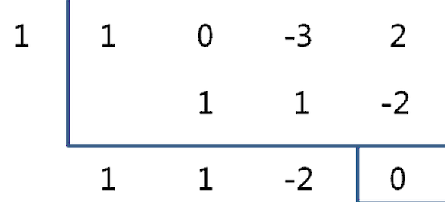
\includegraphics[width=0.6\textwidth]{03_factorization}
\end{figure}
\[x^3-3x+2=(x-1)(x^2+x-2)\]
를 얻는다.
\(x^2+x-2\)는 더 인수분해될 수 있다.
즉 \(x^2+x-2=(x+2)(x-1)\)이다.
따라서
\[x^3-3x+2=(x-1)(x+2)(x-1)=(x-1)^2(x+2)\]
이다.

%%%
\section{복소수}

%%
\subsection{복소수}

%
\defi{허수단위}
제곱해서 \(-1\)이 되는 수를 \(i\)라고 쓴다.
따라서 \(i^2=-1\)이고 \(i=\sqrt{-1}\)이다.

%
\defi{복소수}
실수 \(a\), \(b\)에 대해 \(a+bi\)꼴로 이루어진 수를 \textbf{복소수}라고 한다.
예를 들어 \(1+i\), \(2-3i\), \(-2i\), \(3\) 등은 모두 복소수이다.
이때 \(a\)를 \textbf{실수부분}, \(b\)를 \textbf{허수부분}이라고 부른다.
예를 들어 \(2-3i\)의 실수부분은 \(2\)이고, 허수부분은 \(-3\)이다.

복소수 중에서 \(b\neq0\)인 수를 \textbf{허수}라고 한다.
예를 들어 \(1+i\), \(2-3i\), \(-2i\)는 허수이다.
반면 \(3\)은 실수이다.
허수 중에서 \(a=0\)인 수를 \textbf{순허수}라고 한다.
예를 들어 \(-2i\)는 순허수이다.
반면 \(1+i\), \(2-3i\)는 순허수가 아닌 허수이다.

%
\defi{켤레복소수}
복소수 \(a+bi\)에 대해서 \(a-bi\)를 \(a+bi\)의 \textbf{켤레복소수}라고 한다.
예를 들어 \(1+i\)의 켤레복소수는 \(1-i\)이고 \(2-3i\)의 켤레복소수는 \(2+3i\)이다.
또 \(-2i\)의 켤레복소수는 \(2i\)이고 \(3\)의 켤레복소수는 \(3\)이다.

%
\defi{}
두 복소수 \(a+bi\), \(c+di\)에 대해서 \(a=c\), \(b=d\)이면
\[a+bi=c+di\]
이다.

%
\exam{}
(1)
\[x+yi=3+2i\]
가 성립하면 \(x=3\), \(y=2\)이다.

(2)
\[2x+2i=-4+yi\]
가 성립하면 \(2x=-4\), \(2=y\)이다.
따라서 \(x=-2\), \(y=2\)이다.

(3)
\[(x+y)+(x-y)i=2+4i\]
가 성립하면 \(x+y=2\), \(x-y=4\)이다.
따라서 \(x=3\), \(y=-1\)이다.

%%
\subsection{복소수의 사칙연산}
복소수를 더하거나 빼거나 곱하거나 나눌 때에는 실수에서와 똑같이 교환법칙과 결합법칙, 분배법칙을 잘 적용해나가면서 \(i^2=-1\)를 주의하면서 계산하면 된다.

\exam{}
\(2+i\)와 \(3+2i\)에 대해 우선 덧셈과 뺄셈, 곱셈을 해보자.
\begin{align*}
(2+i)+(3+2i)&=2+i+3+2i=5+3i\\
(2+i)-(3+2i)&=2+i-3-2i=-1-i\\
(2+i)\times(3+2i)&=6+4i+3i+2i^2\\
&=6+4i+3i-2\\
&=4+7i
\end{align*}
이다.

나눗셈을 할 때에는, 분모를 실수로 만들어줘야 한다.
이를 위해 분모의 켤레복소수를 분모와 분자에 각각 곱해줘야 한다.
이 과정을 \textbf{분모의 실수화}라고 한다.
\begin{align*}
(2+i)\div(3+2i)
&=\frac{2+i}{3+2i}\\
&=\frac{(2+i)(3-2i)}{(3+2i)(3-2i)}\\
&=\frac{6-4i+3i-2i^2}{9-6i+6i-4i^2}\\
&=\frac{6-4i+3i+2}{9-6i+6i+4}\\
&=\frac{8-i}{13}\\
&=\frac8{13}-\frac1{13}i.
\end{align*}

%
\defi{음수의 제곱근}
\(a>0\)일 때,
\[\sqrt{-a}=\sqrt ai\]
이다.

%
\exam{}
(1) \(\sqrt{-3}=\sqrt3i\).

(2) \(\sqrt{-4}=\sqrt4i=2i\).

(3) \(\sqrt{-12}=\sqrt{12}i=2\sqrt3i\)이다.

%%%
\section{이차방정식}

%%
\subsection{이차방정식}

%
\defi{이차방정식}
\(a\), \(b\), \(c\)가 실수이고 \(a\neq0\)일 때,
\[ax^2+bx+c=0\]
꼴로 변형될 수 있는 방정식을 \textbf{이차방정식}이라고 한다.

%
\exam{}
(1) \(2x^2-3x+1=0\)은 \(a=2\), \(b=3\), \(c=-1\)이므로 이차방정식이다.

(2) \(x^2+1=0\)은 \(a=1\), \(b=0\), \(c=1\)이므로 이차방정식이다.

(3) \(x^2=-x\)는 \(x^2+x=0\)으로 변형될 수 있고 이 때 \(a=1\), \(b=1\), \(c=0\)이므로 이차방정식이다.

(4) \(2x+1=0\)은 \(a=0\), \(b=2\), \(c=1\)이므로 이차방정식이 아니다.

(5) \(x^2+2x+1=x^2+2x+1\)은 \(0=0\)으로 변형될 수 있고 이때 \(a=0\), \(b=0\), \(c=0\)이므로 이차방정식이 아니다.
이 경우 이 식은 항등식이다.

(6) \(x^2+3x+2=(x+1)^2\)은 \(2x+1=0\)으로 변형될 수 있고 이때 \(a=0\), \(b=2\), \(c=1\)이므로 이차방정식이 아니다.

%
\defi{이차방정식의 근}
이차방정식 \(ax^2+bx+c=0\)에서 \(x\)의 값에 따라 등식
\[ax^2+bx+c=0\]
이 성립하기도 하고 성립하지 않기도 한다.
등식 \(ax^2+bx+c=0\)을 성립하도록 만드는 \(x\)의 값을 이 \textbf{이차방정식의 근}(또는 해)이라고 한다.

또 이차방정식의 근을 구하는 과정을 \textbf{이차방정식을 푼다}고 말한다.

%
\exam{}
이차방정식
\[2x^2-3x+1=0\]
에 \(x=0\)을 넣으면
\(0-0+1\neq0\)이다.
따라서 \(0\)은 이 이차방정식의 근이 아니다.

\(x=1\)을 넣으면
\(2-3+1=0\)이다.
따라서 \(1\)은 이 이차방정식의 근이다.

%%
\subsection{이차방정식의 풀이}

%
\theo{이차방정식의 근의 공식}
이차방정식 \(ax^2+bx+c=0\)의 근은
\[x=\frac{-b\pm\sqrt{b^2-4ac}}{2a}\]
이다.

%
\exam{이차방정식의 풀이(1)}\label{quad_1}
이차방정식
\[x^2+2x-3=0\]
을 풀어보자.

(1) 인수분해를 이용한 방법 :
좌변을 인수분해하면 
\[(x+3)(x-1)=0\]
이 된다.
따라서 \(x+3=0\)이거나 \(x-1=0\)이다.
그러므로 \(x=-3\)이거나 \(x=1\)이다.

(2) 완전제곱식을 이용한 방법 :
\(2px=2x\)이므로 \(p=1\)이다.
\[(x+1)^2=x^2+2x+1\]
이므로 원래 식의 상수항을 우변으로 옮기고 정리하면
\begin{align*}
x^2+2x&=3\\
x^2+2x+1&=3+1\\
(x+1)^2=4\\
x+1=\pm\sqrt4\\
x+1=\pm2\\
x=-1\pm2
\end{align*}
이다.
따라서 \(x=-1+2=1\)이거나 \(x=-1-2=-3\)이다.

(3) 근의 공식을 이용한 방법 :
\(a=1\), \(b=2\), \(c=-3\)이므로
\begin{align*}
x
&=\frac{-2\pm\sqrt{2^2-4\cdot1\cdot(-3)}}{2\cdot1}\\
&=\frac{-2\pm\sqrt{16}}2\\
&=\frac{-2\pm4}2
\end{align*}
이다.
따라서 \(x=\frac{-2+4}2=\frac22=1\)이거나 \(x=\frac{-2-4}2=\frac{-6}2=-3\)이다.

%
\exam{이차방정식의 풀이(2)}\label{quad_2}
이차방정식 \[x^2+6x+9=0\]을 풀어보자.

(1) 인수분해를 이용한 방법 :
좌변을 인수분해하면 
\[(x+3)^2=0\]
이 된다.
따라서 \(x+3=0\)이다.
그러므로 \(x=-3\)이다.

(2) 완전제곱식을 이용한 방법 :
\(2px=6x\)이므로 \(p=3\)이다.
\[(x+3)^2=x^2+6x+9\]
이므로 원래 식의 상수항을 우변으로 옮기고 정리하면
\begin{align*}
x^2+6x&=-9\\
x^2+6x+9&=-9+9\\
(x+3)^2=0\\
x+3=\pm\sqrt0\\
x+3=\pm0\\
x+3=0\\
x=-3
\end{align*}
이다.

(3) 근의 공식을 이용한 방법 :
\(a=1\), \(b=6\), \(c=9\)이므로
\begin{align*}
x
&=\frac{-6\pm\sqrt{6^2-4\cdot1\cdot9}}{2\cdot1}\\
&=\frac{-6\pm\sqrt{0}}2\\
&=\frac{-6\pm0}2\\
&=\frac{-6}2\\
&=-3
\end{align*}
이다.

%
\exam{이차방정식의 풀이(3)}\label{quad_3}
이차방정식 \[x^2-2x+3=0\]을 풀어보자.

(1) 인수분해를 이용한 방법 :
인수분해가 쉽게 되지 않는다.
따라서 인수분해를 이용한 방법을 사용할 수 없다.

(2) 완전제곱식을 이용한 방법 :
\(2px=-2x\)이므로 \(p=-1\)이다.
\[(x-1)^2=x^2-2x+1\]
이므로 원래 식의 상수항을 우변으로 옮기고 정리하면
\begin{align*}
x^2-2x&=-3\\
x^2-2x+1&=-3+1\\
(x-1)^2=-2\\
x-1=\pm\sqrt{-2}\\
x-1=\pm\sqrt{2}i\\
x=1\pm\sqrt2i
\end{align*}
이다.
따라서 \(x=1+\sqrt2i\)이거나 \(x=1-\sqrt2i\)이다.

(3) 근의 공식을 이용한 방법 :
\(a=1\), \(b=-2\), \(c=3\)이므로
\begin{align*}
x
&=\frac{-(-2)\pm\sqrt{(-2)^2-4\cdot1\cdot3}}{2\cdot1}\\
&=\frac{2\pm\sqrt{-8}}2\\
&=\frac{2\pm\sqrt8i}2\\
&=\frac{2\pm2\sqrt2i}2
\end{align*}
이다.
따라서 \(x=\frac{2+2\sqrt2i}2=\frac22+\frac{2\sqrt2}2i=1+\sqrt2i\)이거나 \(x=\frac{2-2\sqrt2i}2=\frac22-\frac{2\sqrt2}2i=1-\sqrt2i\)이다.

이 경우 근은 실수가 아니라 허수이다.
이처럼 허수인 근을 \textbf{허근}이라고 하고, 반면에 예제 \ref{quad_1}, \ref{quad_2}에서처럼 실수인 근을 \textbf{실근}이라고 한다.

%%
\subsection{판별식}
예제 \ref{quad_1}, \ref{quad_2}, \ref{quad_3}에서 보듯, 이차방정식의 해는 실수가 될 수도 있고 허수가 될 수도 있다.
또 해의 갯수가 두 개 일 수도 있고 한 개일 수도 있다.
이런 차이가 발생하는 까닭은 근의 공식에서 \(\sqrt{b^2-4ac}\)의 값이 0이 될 수도 있고 0이 아닌 실수가 될 수도 있고 허수가 될 수도 있기 때문이다.
따라서 판별식 \(D\)를 다음과 같이 정의하고 이차방정식의 실수인 근의 갯수를 판별하는 용도로 쓴다.

%
\defi{판별식}
이차방정식 \(ax^2+bx+c=0\)에 대한 판별식은
\[D=b^2-4ac\]
이다.

%
\theo{이차방정식의 근의 판별}\label{det.}
이차방정식 \(ax^2+bx+c=0\)에서\\
(1) \(D>0\)이면 이차방정식은 두 실근을 가진다(예제 \ref{quad_1}).\\
(2) \(D=0\)이면 이차방정식은 한 실근을 가진다(예제 \ref{quad_2}).\\
(3) \(D<0\)이면 이차방정식은 두 허근을 가진다(예제 \ref{quad_3}).

(1)의 경우 의미를 강조하기 위해 ``\text{서로 다른} 두 실근을 가진다''라고 말하기도 한다.
또 (2)의 경우에는 `중복된 근'이라는 의미에서 ``\text{\textbf{중근}}을 가진다''고 말하기도 한다.

%
\exam{}
예제 \ref{quad_1}에서 이차방정식 \(x^2+2x-3=0\)은 두 실근 \(1\), \(-3\)을 가졌다.
실제로 판별식을 계산해보면
\(a=1\), \(b=2\), \(c=-3\)
이므로
\[D=2^2-4\cdot1\cdot(-3)=16>0\]
이다.
따라서 두 실근을 가지는 것이 맞다.

예제 \ref{quad_2}에서 이차방정식 \(x^2+6x+9=0\)은 한 실근 \(-3\)을 가졌다.
실제로 판별식을 계산해보면
\(a=1\), \(b=6\), \(c=9\)
이므로
\[D=6^2-4\cdot1\cdot9=0\]
이다.
따라서 한 실근을 가지는 것이 맞다.

예제 \ref{quad_3}에서 이차방정식 \(x^2+2x+3=0\)은 두 허근 \(1+\sqrt2i\), \(1-\sqrt2i\)를 가졌다.
실제로 판별식을 계산해보면
\(a=1\), \(b=2\), \(c=3\)
이므로
\[D=2^2-4\cdot1\cdot3=-8<0\]
이다.
따라서 두 허근을 가지는 것이 맞다.

%%
\subsection{근과 계수와의 관계}

이차방정식 \(ax^2+bx+c=0\)의 두 근을 \(\alpha\)와 \(\beta\)라고 하자.
정리 \ref{det.}에 의해
\(D>0\)이면 두 근은 실수이고 \(\alpha\neq\beta\)이다.
\(D=0\)이면 두 근은 실수이고 \(\alpha=\beta\)이다.
\(D<0\)이면 두 근은 허수이고 \(\alpha\neq\beta\)이다.
이때 \(\alpha\), \(\beta\)와 \(a\), \(b\), \(c\) 사이에 다음 관계가 성립한다.

%
\theo{}
\[
\alpha+\beta=-\frac ba,
\quad
\alpha\beta=\frac ca
\]
\begin{proof}
근의 공식에 의해
\[
\alpha=\frac{-b+\sqrt{b^2-4ac}}{2a}
,\quad
\beta=\frac{-b-\sqrt{b^2-4ac}}{2a}
\]
이다(또는 그 반대이다).
이를 바탕으로 \(\alpha+\beta\)와 \(\alpha\beta\)를 계산하면 된다.
\end{proof}

%%%
\section{이차방정식과 이차함수}

%%
\subsection{이차함수}

%
\defi{이차함수}
함수 \(f\)가
\[f(x)=ax^2+bx+c\]
꼴로 정의되어 있으면(\(a\neq0\)) \(f\)를 \textbf{이차함수}라고 부른다.

\(f(x)=ax^2+bx+c\)를 가끔씩은
\[y=ax^2+bx+c\]
로 쓰기도 한다.

%
\exam{}
(1) \(f(x)=3x^2+2x+1\)은 \(a=3\), \(b=2\), \(c=1\)인 이차함수이다.

(2) \(y=2x^2-1\)은 \(a=2\), \(b=0\), \(c=-1\)인 이차함수이다.

(3) \(f(x)=4x+1\)은 \(a=0\), \(b=4\), \(c=1\)이므로 이차함수가 아니다.

(4) \(y=3\)은 \(a=0\), \(b=0\), \(c=3\)이므로 이차함수가 아니다.

%
\defi{이차함수의 그래프}
이차함수 \(y=ax^2+bx+c\)의 그래프는
\[y=ax^2+bx+c\]
을 만족하는 점 \((x,y)\)들의 집합을 말한다.

%
\exam{}
\(y=x^2\)의 그래프는
\[y=x^2\]
을 만족하는 점 \((x,y)\)들의 집합을 말한다.

예를 들어 \((0,0)\)은 \(0=0^2\)을 만족하므로 \(y=x^2\)의 그래프의 일부이다.
또 \((1,1)\), \((2,4)\)도 \(1=1^2\), \(4=2^2\)을 만족하므로 \(y=x^2\)의 그래프의 일부이다.
반면 \((1,2)\)는 \(2\neq1^2\)이므로 \(y=x^2\)의 그래프의 점이 아니다.

그래프 위에 있는 점들은 대략
\[(0,0),(1,1),(-1,1),(2,4),(-2,4),(3,9),(-3,9),(4,16),(-4,16),\cdots\]
등이므로 좌표 평면 위에 \(y=x^2\)의 그래프를 나타내면

\begin{figure}[h]
\center
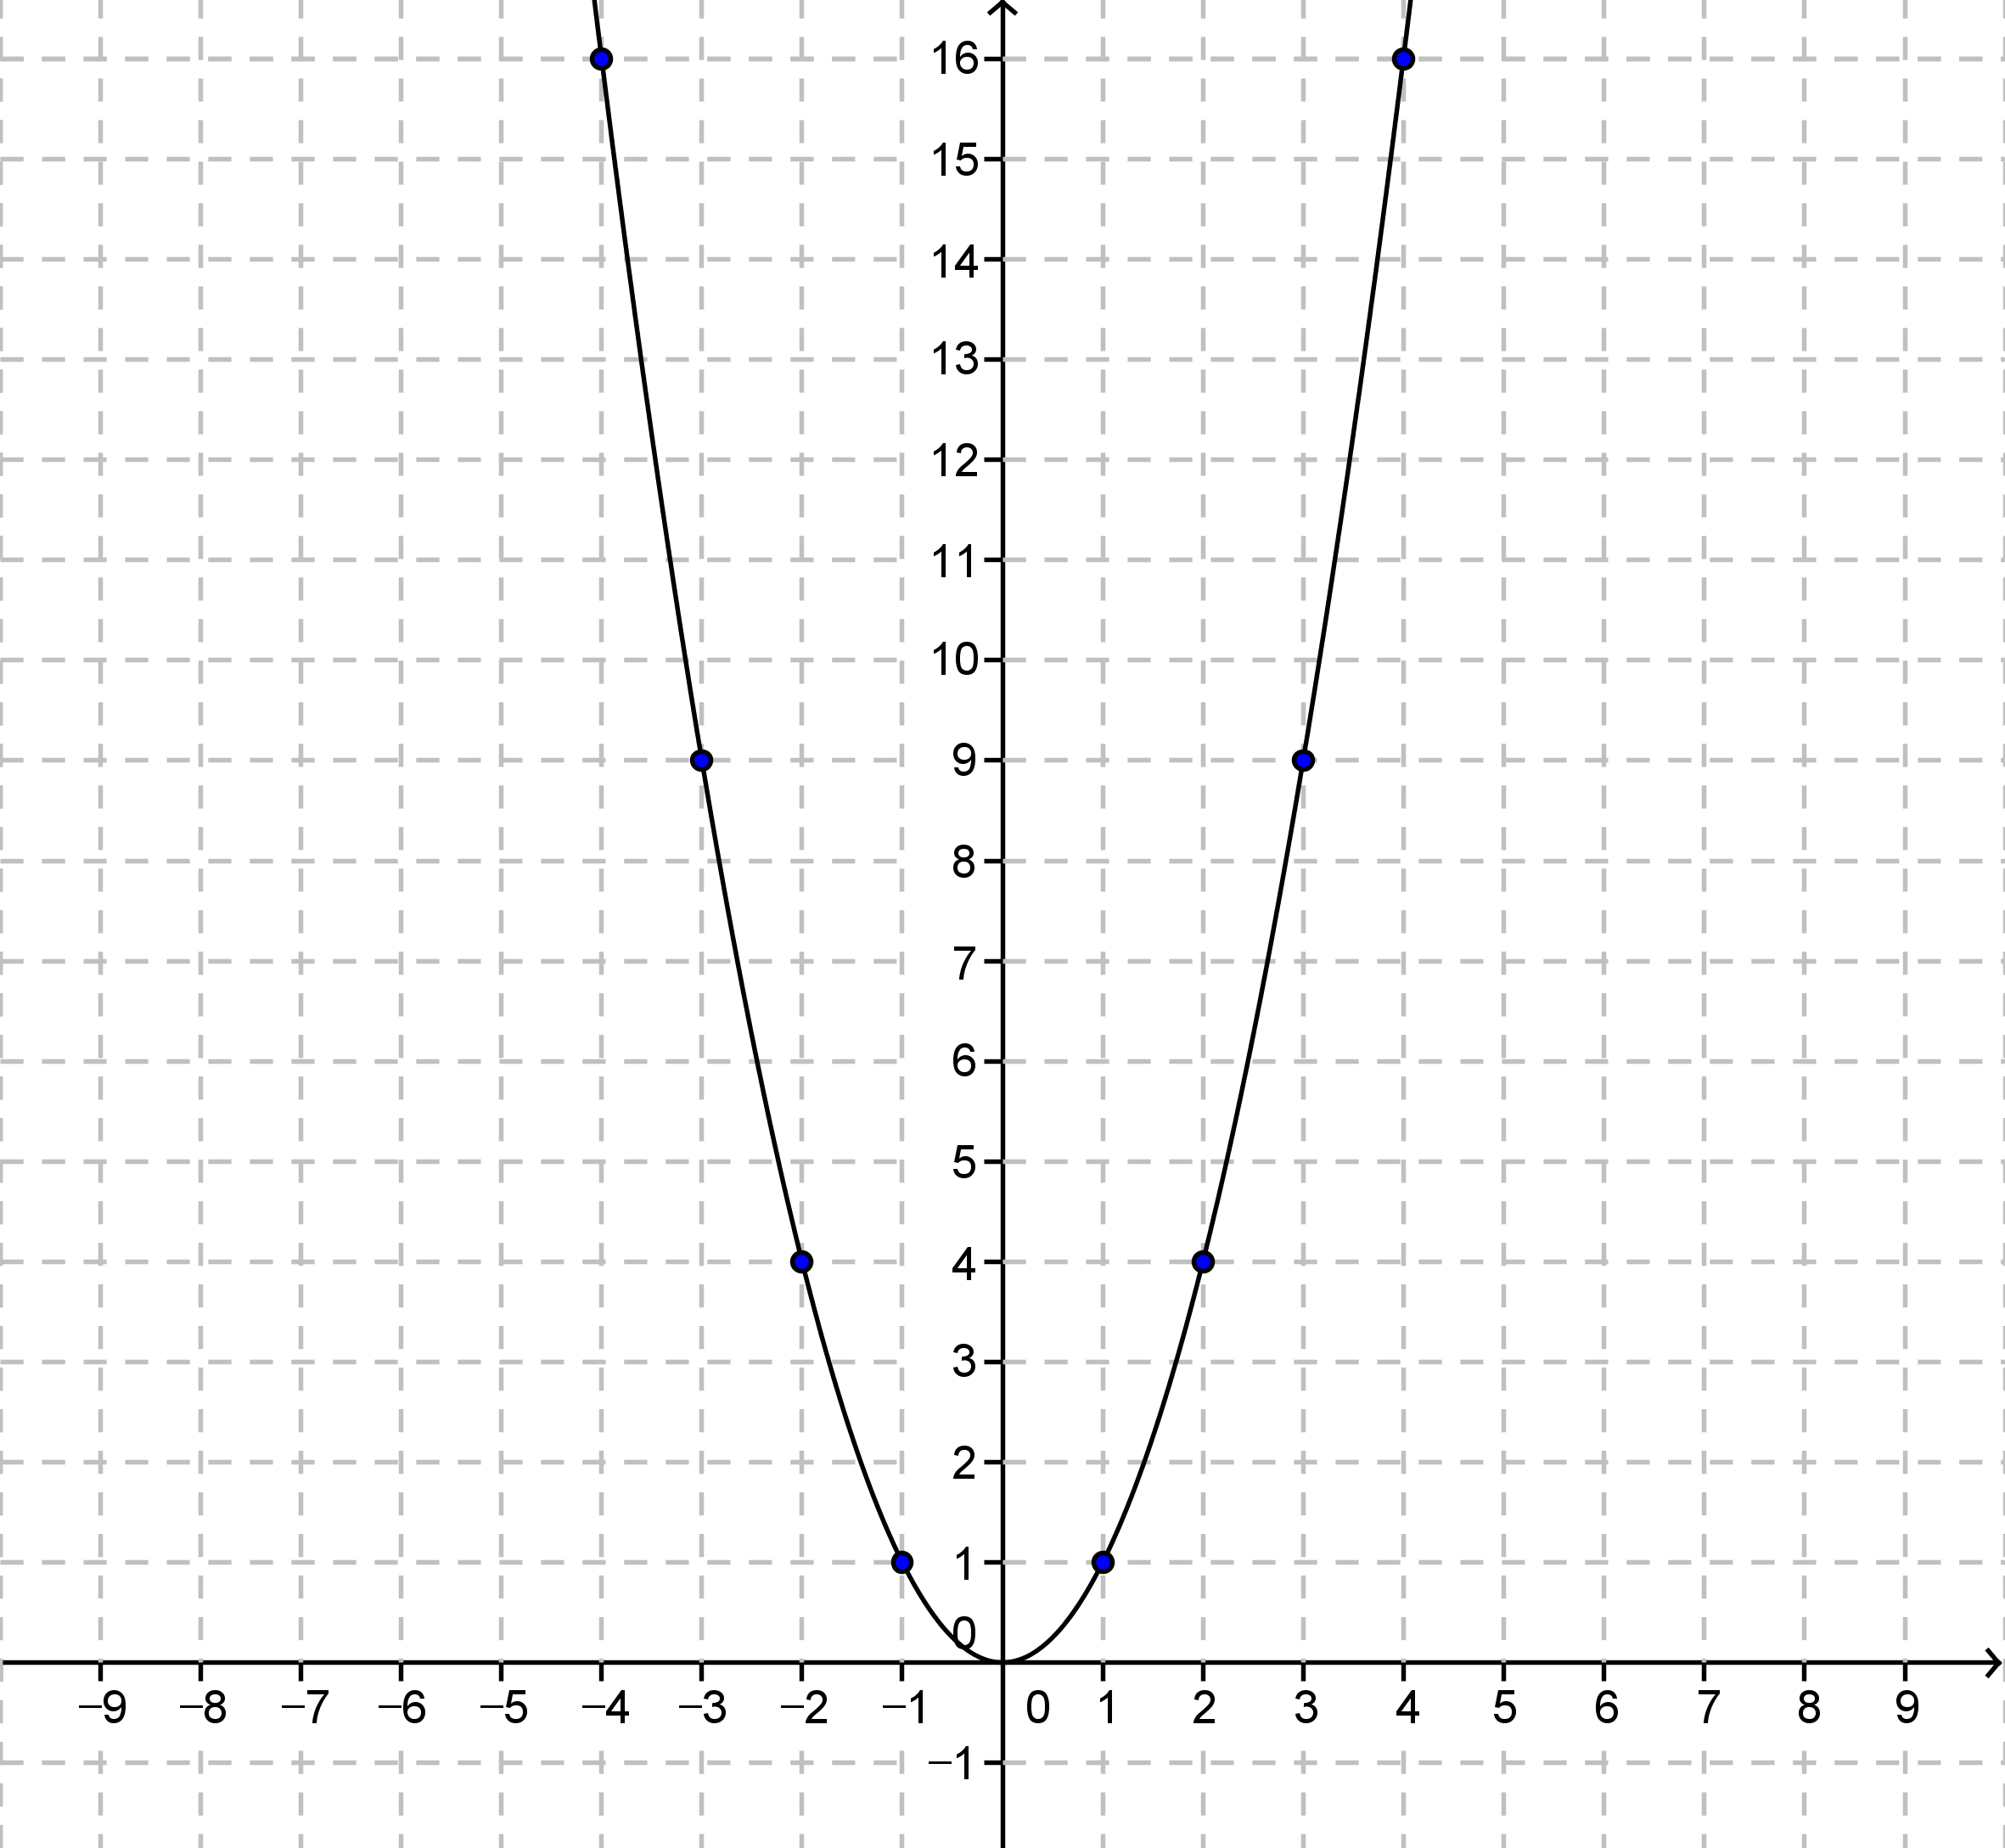
\includegraphics[width=0.5\textwidth]{06_01_y=x^2}
\end{figure}
이다.

%
\theo{}
모든 이차함수
\[y=ax^2+bx+c\]
는
\[y=a(x-p)^2+q\]
꼴로 바꿀 수 있고
이때 이 이차함수의 그래프는 \((p,q)\)를 꼭지점으로 하는 포물선이다.
\(a>0\)이면 그래프는 아래로 볼록이고, \(a<0\)이면 그래프는 위로 볼록이다.

%
\exam{}\label{quad.func.graph_01}
이차함수
\[y=x^2+4x+2\]
의 그래프를 그려보자.
\[2px=4x\]
이므로 \(p=2\)이고
\[(x+2)^2=x^2+4x+4\]
이다.
따라서
\begin{align*}
y
&=x^2+4x+2\\
&=(x^2+4x+4)-4+2\\
&=(x+2)^2-2\\
\end{align*}
이고 \(a=1\), \(p=-2\), \(q=-2\)이다.
그러므로 그래프의 꼭지점은 \((-2,-2)\)이고, \(a>0\)이므로 아래로 볼록이다.

\begin{figure}[h]
\center
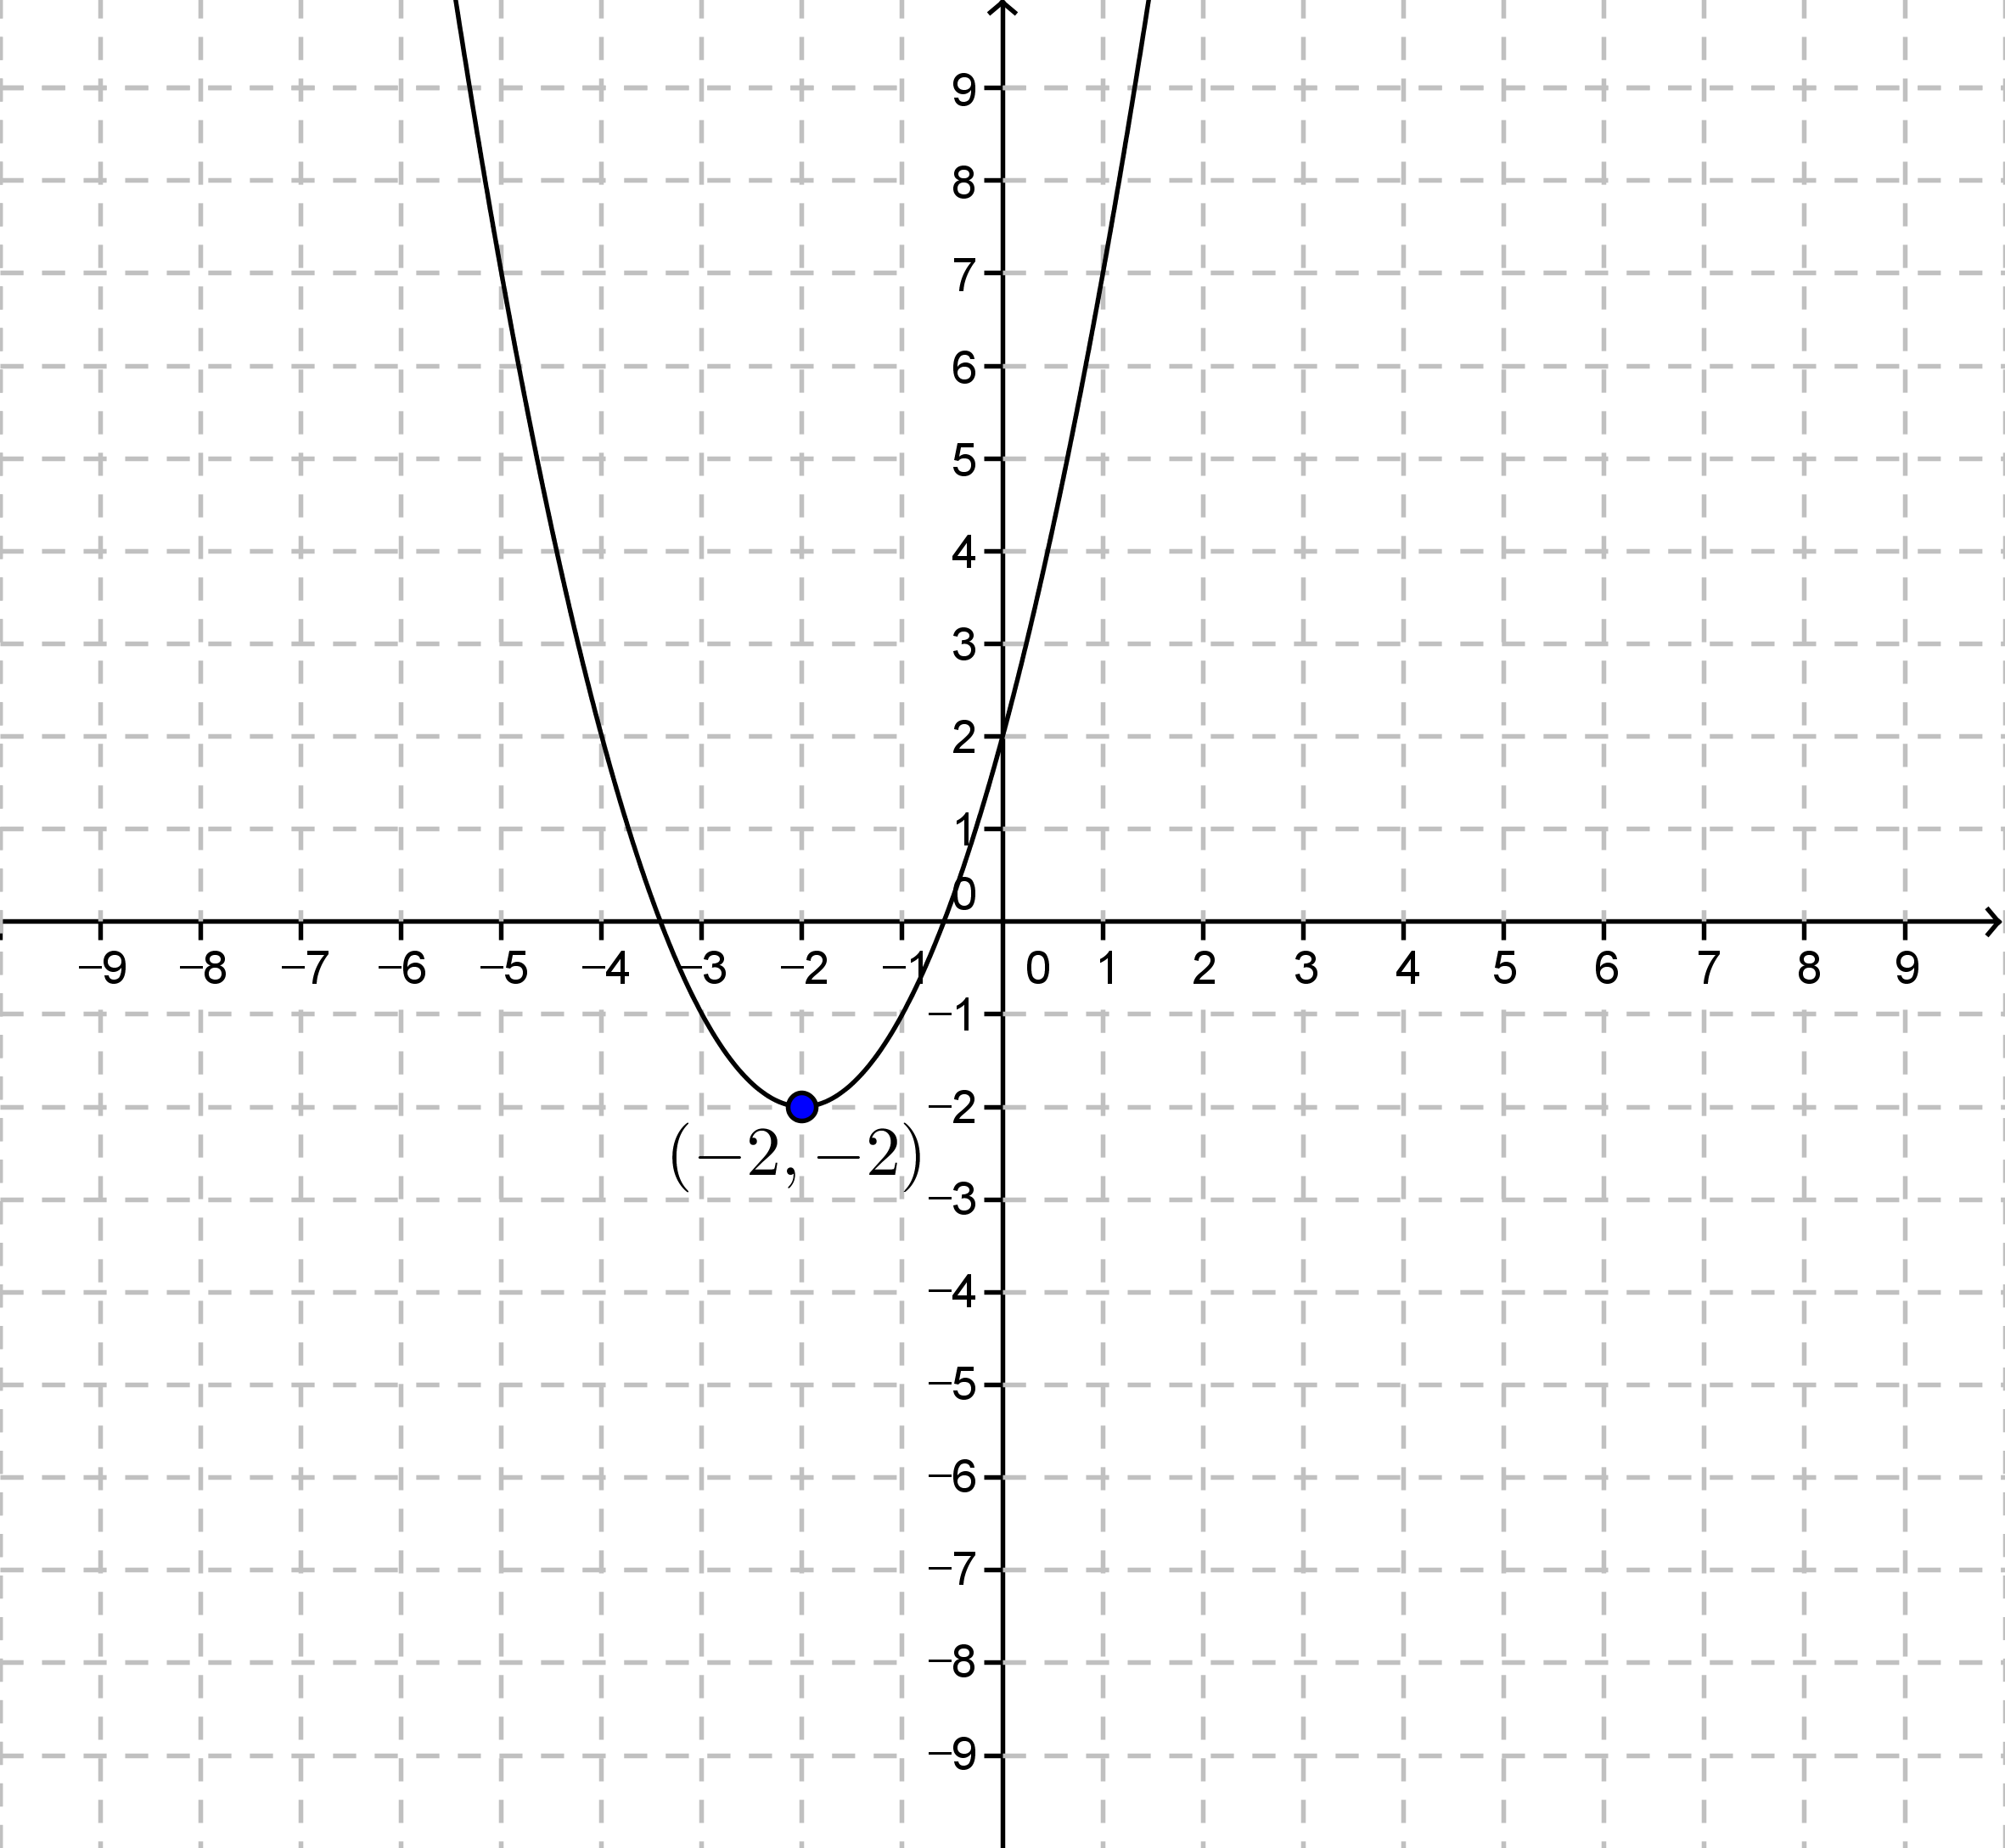
\includegraphics[width=0.5\textwidth]{06_01_y=x^2+4x+2}
\end{figure}

%
\exam{}\label{quad.func.graph_02}
이차함수
\[y=2x^2+8x+8\]
의 그래프를 그려보자.
최고자항 \(2x^2\)의 계수 \(2\)로 묶으면
\begin{align*}
y
&=2x^2+8x+8\\
&=2(x^2+4x)+8
\end{align*}
이다.
\[2px=4x\]
이므로 \(p=2\)이고
\[(x+2)^2=x^2+4x+4\]
이다.
따라서
\begin{align*}
y
&=2(x^2+4x)+8\\
&=2(x^2+4x+4-4)+8\\
&=2(x^2+4x+4)-8+8\\
&=2(x+2)^2
\end{align*}
이고 \(a=2\), \(p=-2\), \(q=0\)이다.
그러므로 그래프의 꼭지점은 \((-2,0)\)이고, \(a>0\)이므로 아래로 볼록이다.

\begin{figure}[h]
\center
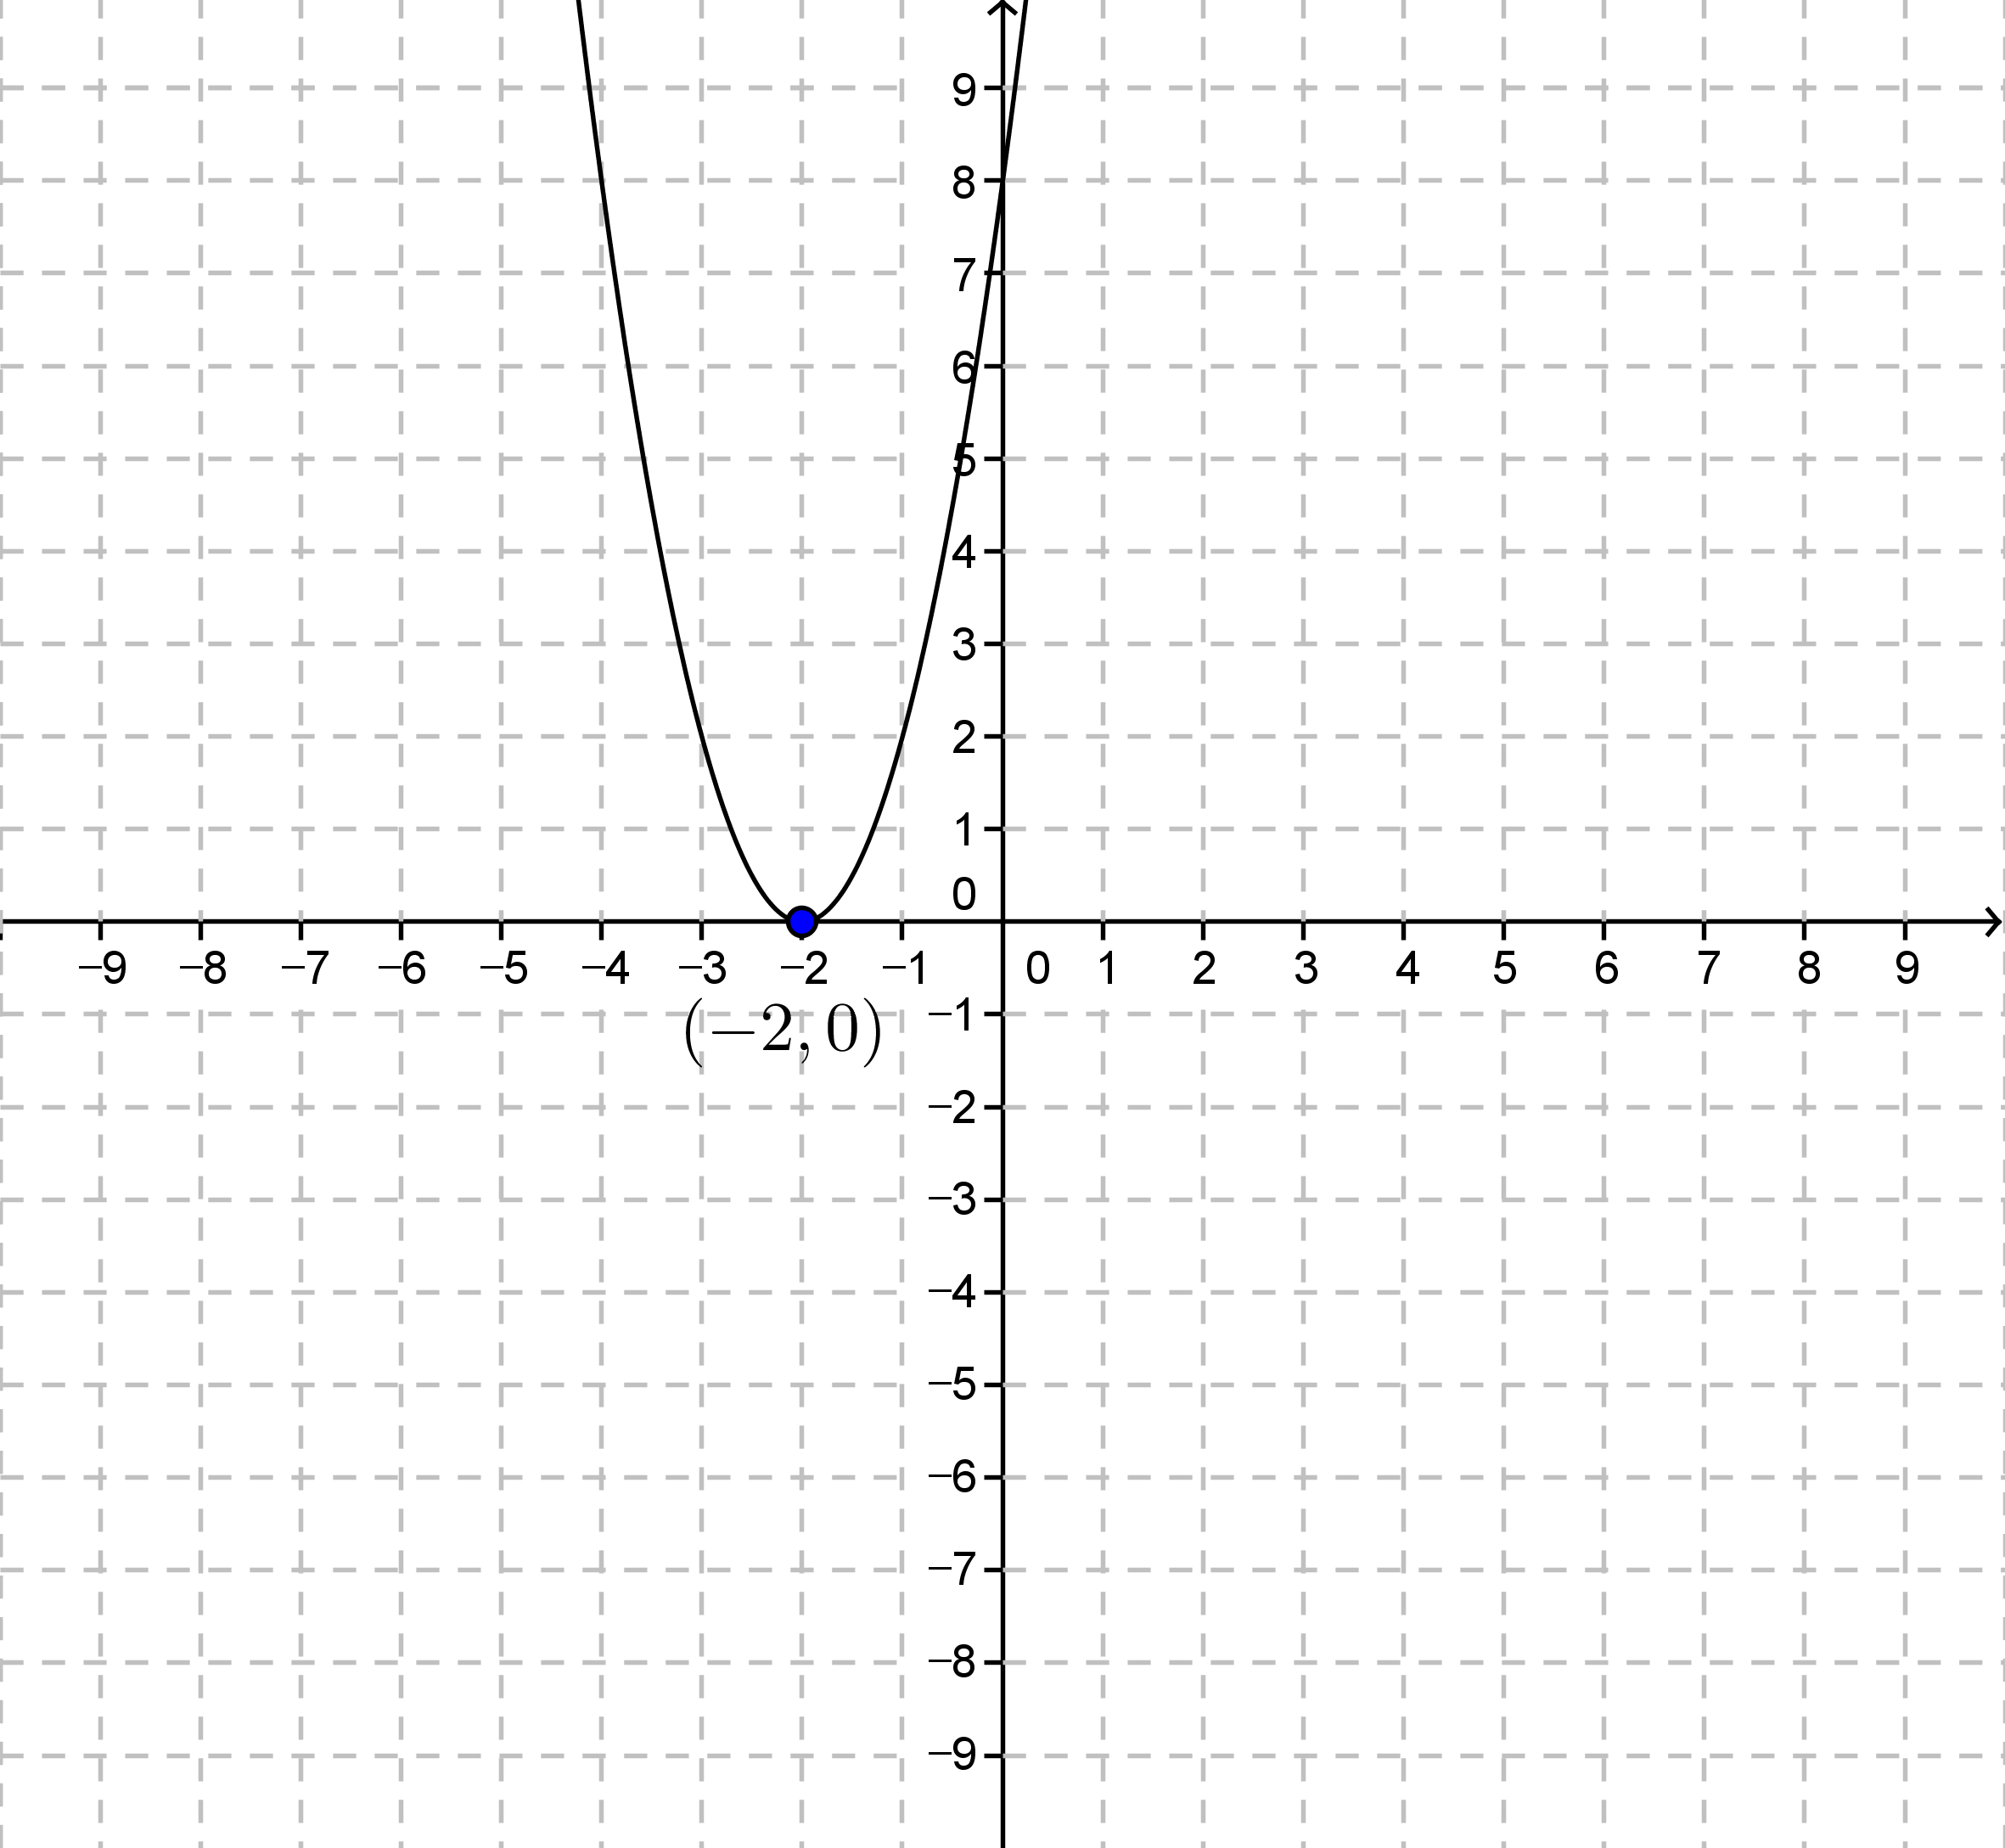
\includegraphics[width=0.5\textwidth]{06_01_y=2x^2+8x+8}
\end{figure}

%
\exam{}\label{quad.func.graph_03}
이차함수
\[y=-2x^2+4x-3\]
의 그래프를 그려보자.
최고자항 \(-2x^2\)의 계수 \(-2\)로 묶으면
\begin{align*}
y
&=-2x^2+4x-3\\
&=-2(x^2-2x)-3
\end{align*}
이다.
\[2px=-2x\]
이므로 \(p=-1\)이고
\[(x-1)^2=x^2-2x+1\]
이다.
따라서
\begin{align*}
y
&=-2(x^2-2x)-3\\
&=-2(x^2-2x+1-1)-3\\
&=-2(x^2-2x+1)+2-3\\
&=-2(x-1)^2-1
\end{align*}
이고 \(a=-2\), \(p=1\), \(q=-1\)이다.
그러므로 그래프의 꼭지점은 \((1,-1)\)이고, \(a<0\)이므로 위로 볼록이다.

\begin{figure}[h]
\center
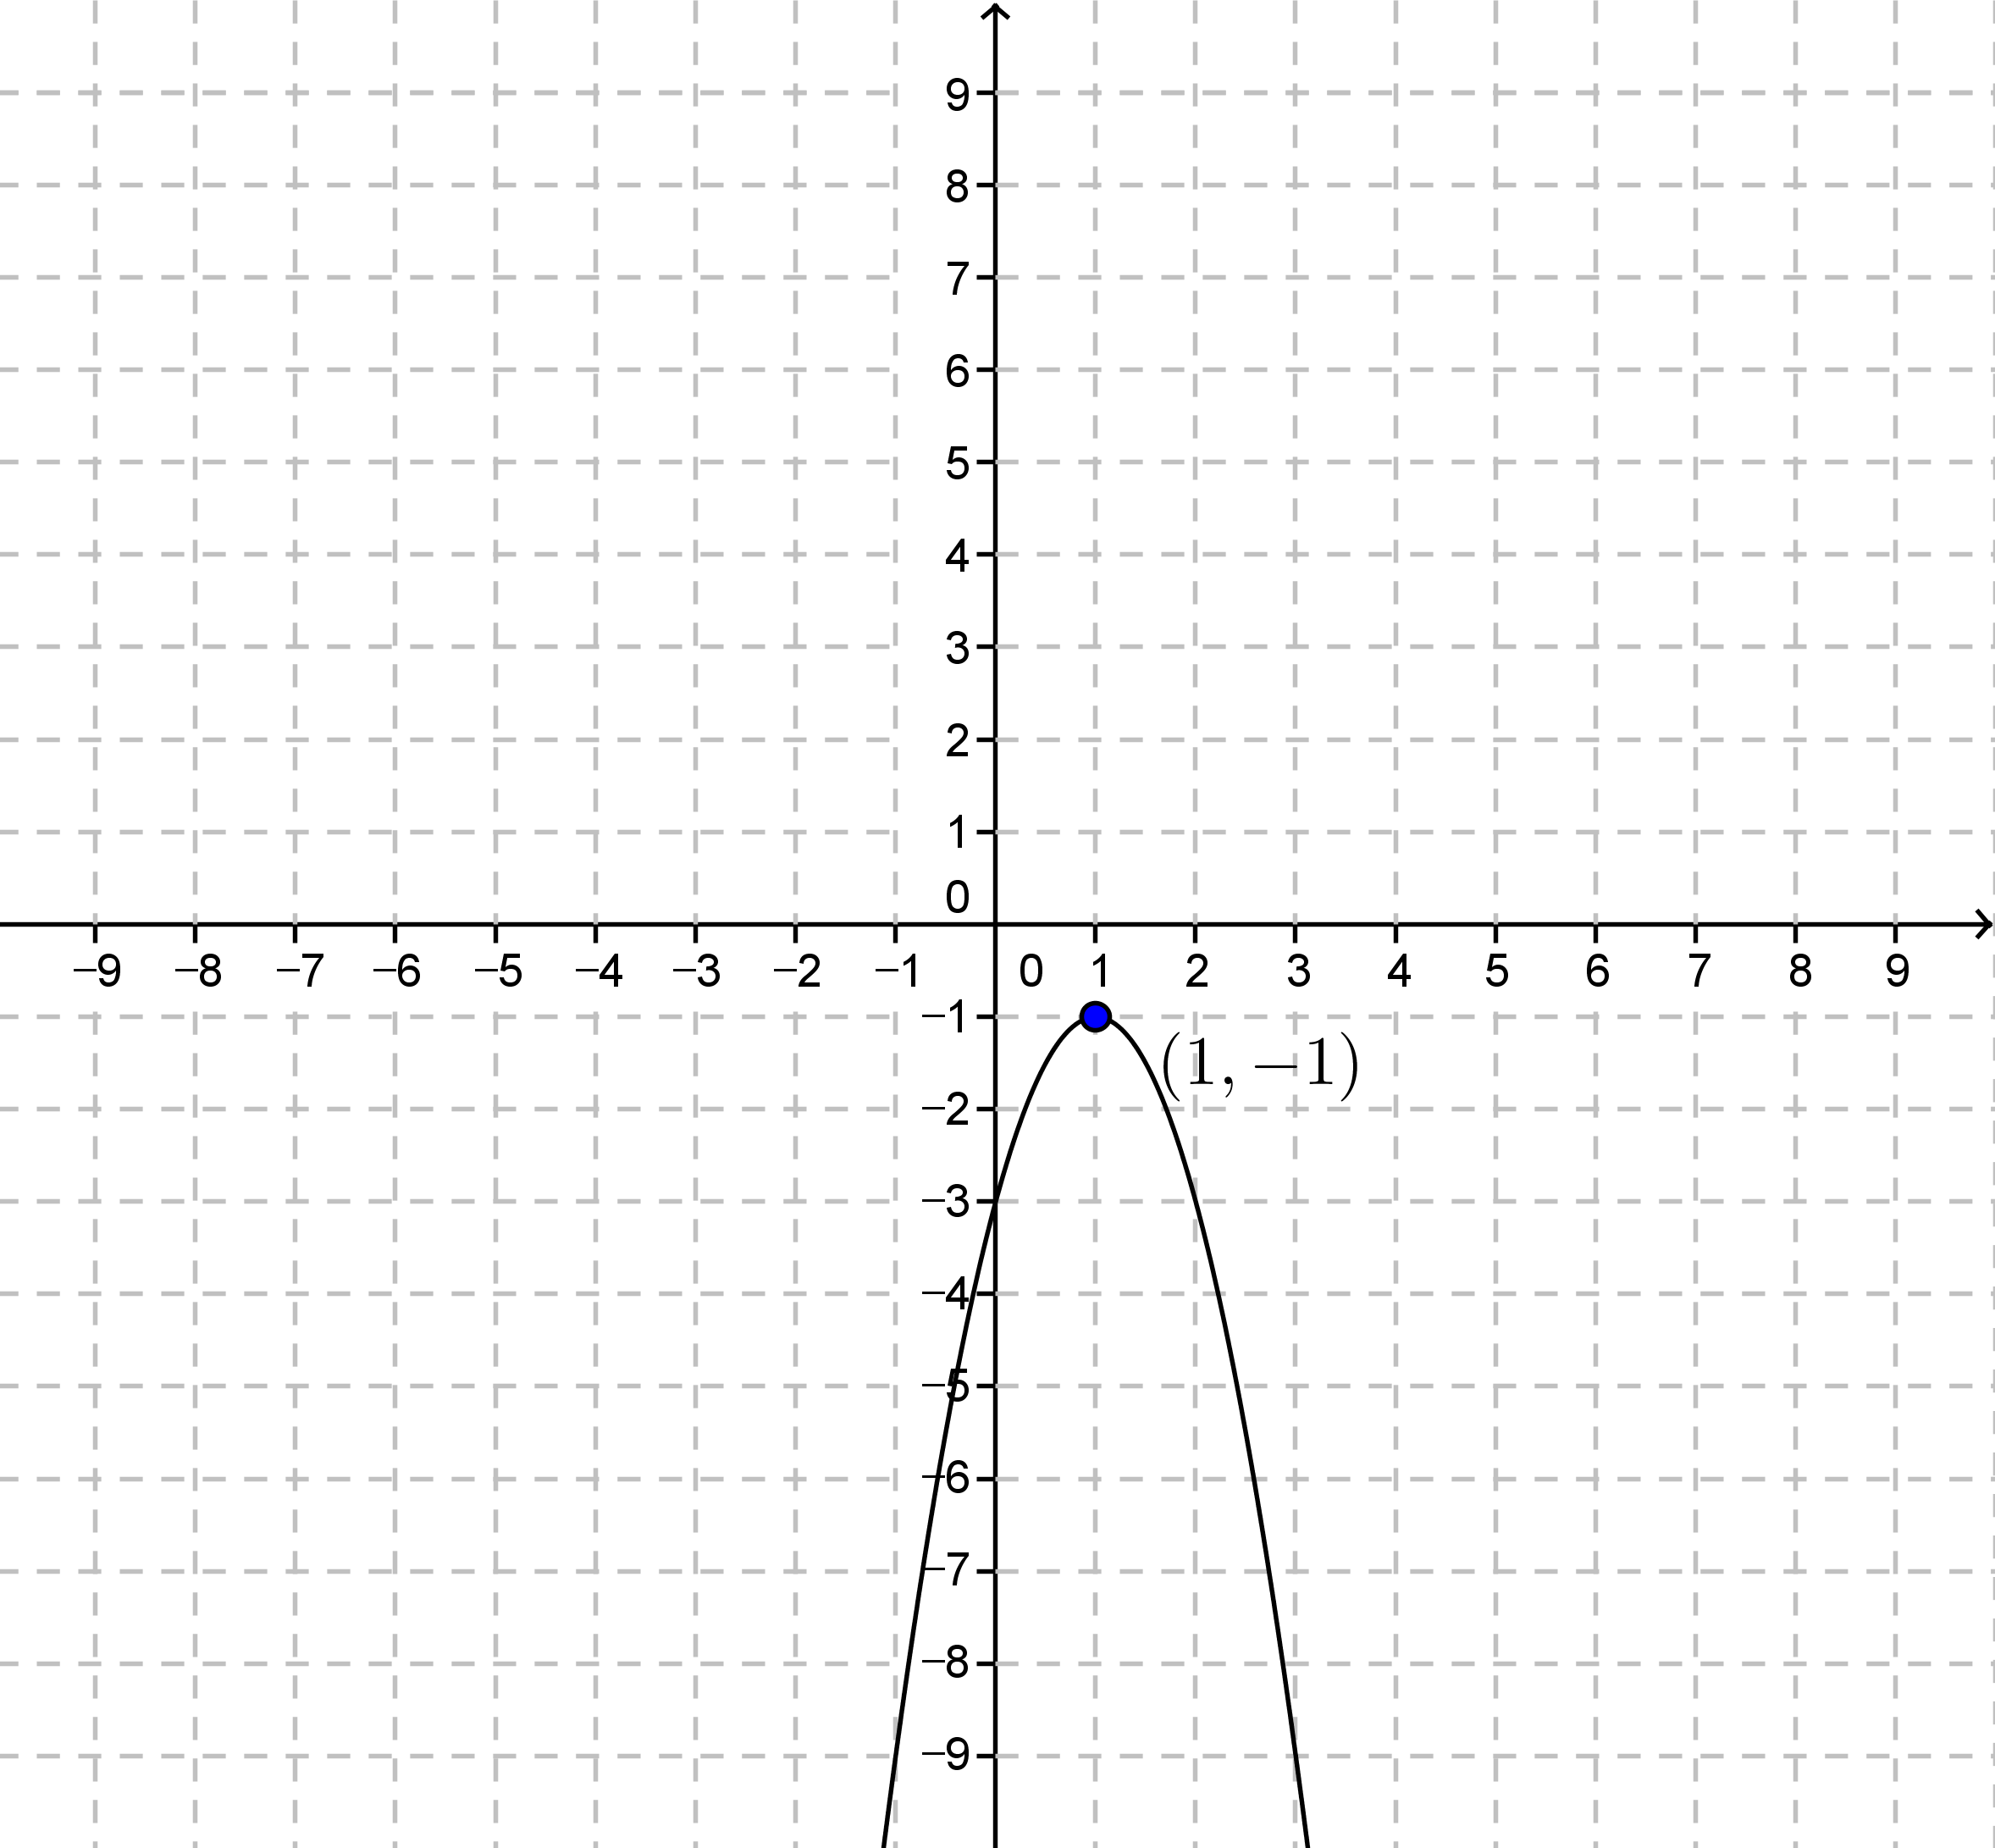
\includegraphics[width=0.5\textwidth]{06_01_y=-2x^2+4x-3}
\end{figure}

%%
\subsection{이차함수의 그래프와 \(x\)축 사이의 위치관계}

%
\theo{}\label{quad.D_01}
이차함수 \(y=ax^2+bx+c\)에 대해서 \(D=b^2-4ac\)이라고 하자.

그러면\\
(1) \(D>0\)이면 이 이차함수의 그래프와 \(x\)축 사이의 교점은 두 개이다.\\
(2) \(D=0\)이면 이 이차함수의 그래프와 \(x\)축 사이의 교점은 한 개이다(접한다).\\
(3) \(D<0\)이면 이 이차함수의 그래프와 \(x\)축 사이의 교점은 없다.

%
\exam{}
예제 \ref{quad.func.graph_01}의
\[y=x^2+4x+2\]
에서 \(a=1\), \(b=4\), \(c=2\)이다.
따라서 \(D=4^2-4\cdot1\cdot2=8>0\)이다. 정리 \ref{quad.D_01}의 (1)에 따르면 이 함수의 그래프와 \(x\)축과의 교점이 두 개여야 한다.
실제로 그래프와 \(x\)축 사이의 교점도 두 개이다.

예제 \ref{quad.func.graph_02}의
\[y=2x^2+8x+8\]
에서 \(a=2\), \(b=8\), \(c=8\)이다.
따라서 \(D=8^2-4\cdot2\cdot8=0\)이다. 정리 \ref{quad.D_01}의 (2)에 따르면 이 함수의 그래프와 \(x\)축과의 교점이 한 개여야 한다.
실제로 그래프와 \(x\)축 사이의 교점도 한 개이다.

예제 \ref{quad.func.graph_03}의
\[y=-2x^2+4x-3\]
에서 \(a=-2\), \(b=4\), \(c=-3\)이다.
따라서 \(D=4^2-4\cdot(-2)\cdot(-3)=16-24=-8<0\)이다. 정리 \ref{quad.D_01}의 (3)에 따르면 이 함수의 그래프와 \(x\)축과의 교점이 없어야 한다.
실제로 그래프와 \(x\)축 사이의 교점은 없다.

%%
\subsection{이차함수의 그래프와 직선 사이의 위치관계}

%
\theo{}
이차함수 \(y=ax^2+bx+c\)의 그래프와 직선 \(y=mx+n\)을 생각하자.
두 식을 연립해서 얻어지는 방정식
\[ax^2+(b-m)x+c-n=0\]
에 대해
\[D=(b-m)^2-4a(c-n)\]
라고 할 때,\\
(1) \(D>0\)이면 이 이차함수의 그래프와 직선 사이의 교점은 두 개이다.\\
(2) \(D=0\)이면 이 이차함수의 그래프와 직선 사이의 교점은 한 개이다(접한다).\\
(3) \(D<0\)이면 이 이차함수의 그래프와 직선 사이의 교점은 없다.

%
\exam{}
이차함수
\[y=x^2+4x+2\]
와 세 개의 직선
\begin{align}
y&=2x\\
y&=2x+1\\
y&=2x+2
\end{align}
을 생각하자.

(1)
\[x^2+4x+2=2x\]
의 우변을 좌변으로 이항하면
\[x^2+2x+2=0\]
이고 \(D=2^2-4\cdot1\cdot2<0\)이다.
따라서 이차함수의 그래프와 직선 \(y=2x\) 사이의 교점은 없다.

(2)
\[x^2+4x+2=2x+1\]
의 우변을 좌변으로 이항하면
\[x^2+2x+1=0\]
이고 \(D=2^2-4\cdot1\cdot1=0\)이다.
따라서 이차함수의 그래프와 직선 \(y=2x+1\) 사이의 교점은 한 개이다.

(3)
\[x^2+4x+2=2x+2\]
의 우변을 좌변으로 이항하면
\[x^2+2x=0\]
이고 \(D=2^2-4\cdot1\cdot0>0\)이다.
따라서 이차함수의 그래프와 직선 \(y=2x+2\) 사이의 교점은 두 개이다.

실제로 그래프들을 모두 그려보면
\begin{figure}[h]
\center
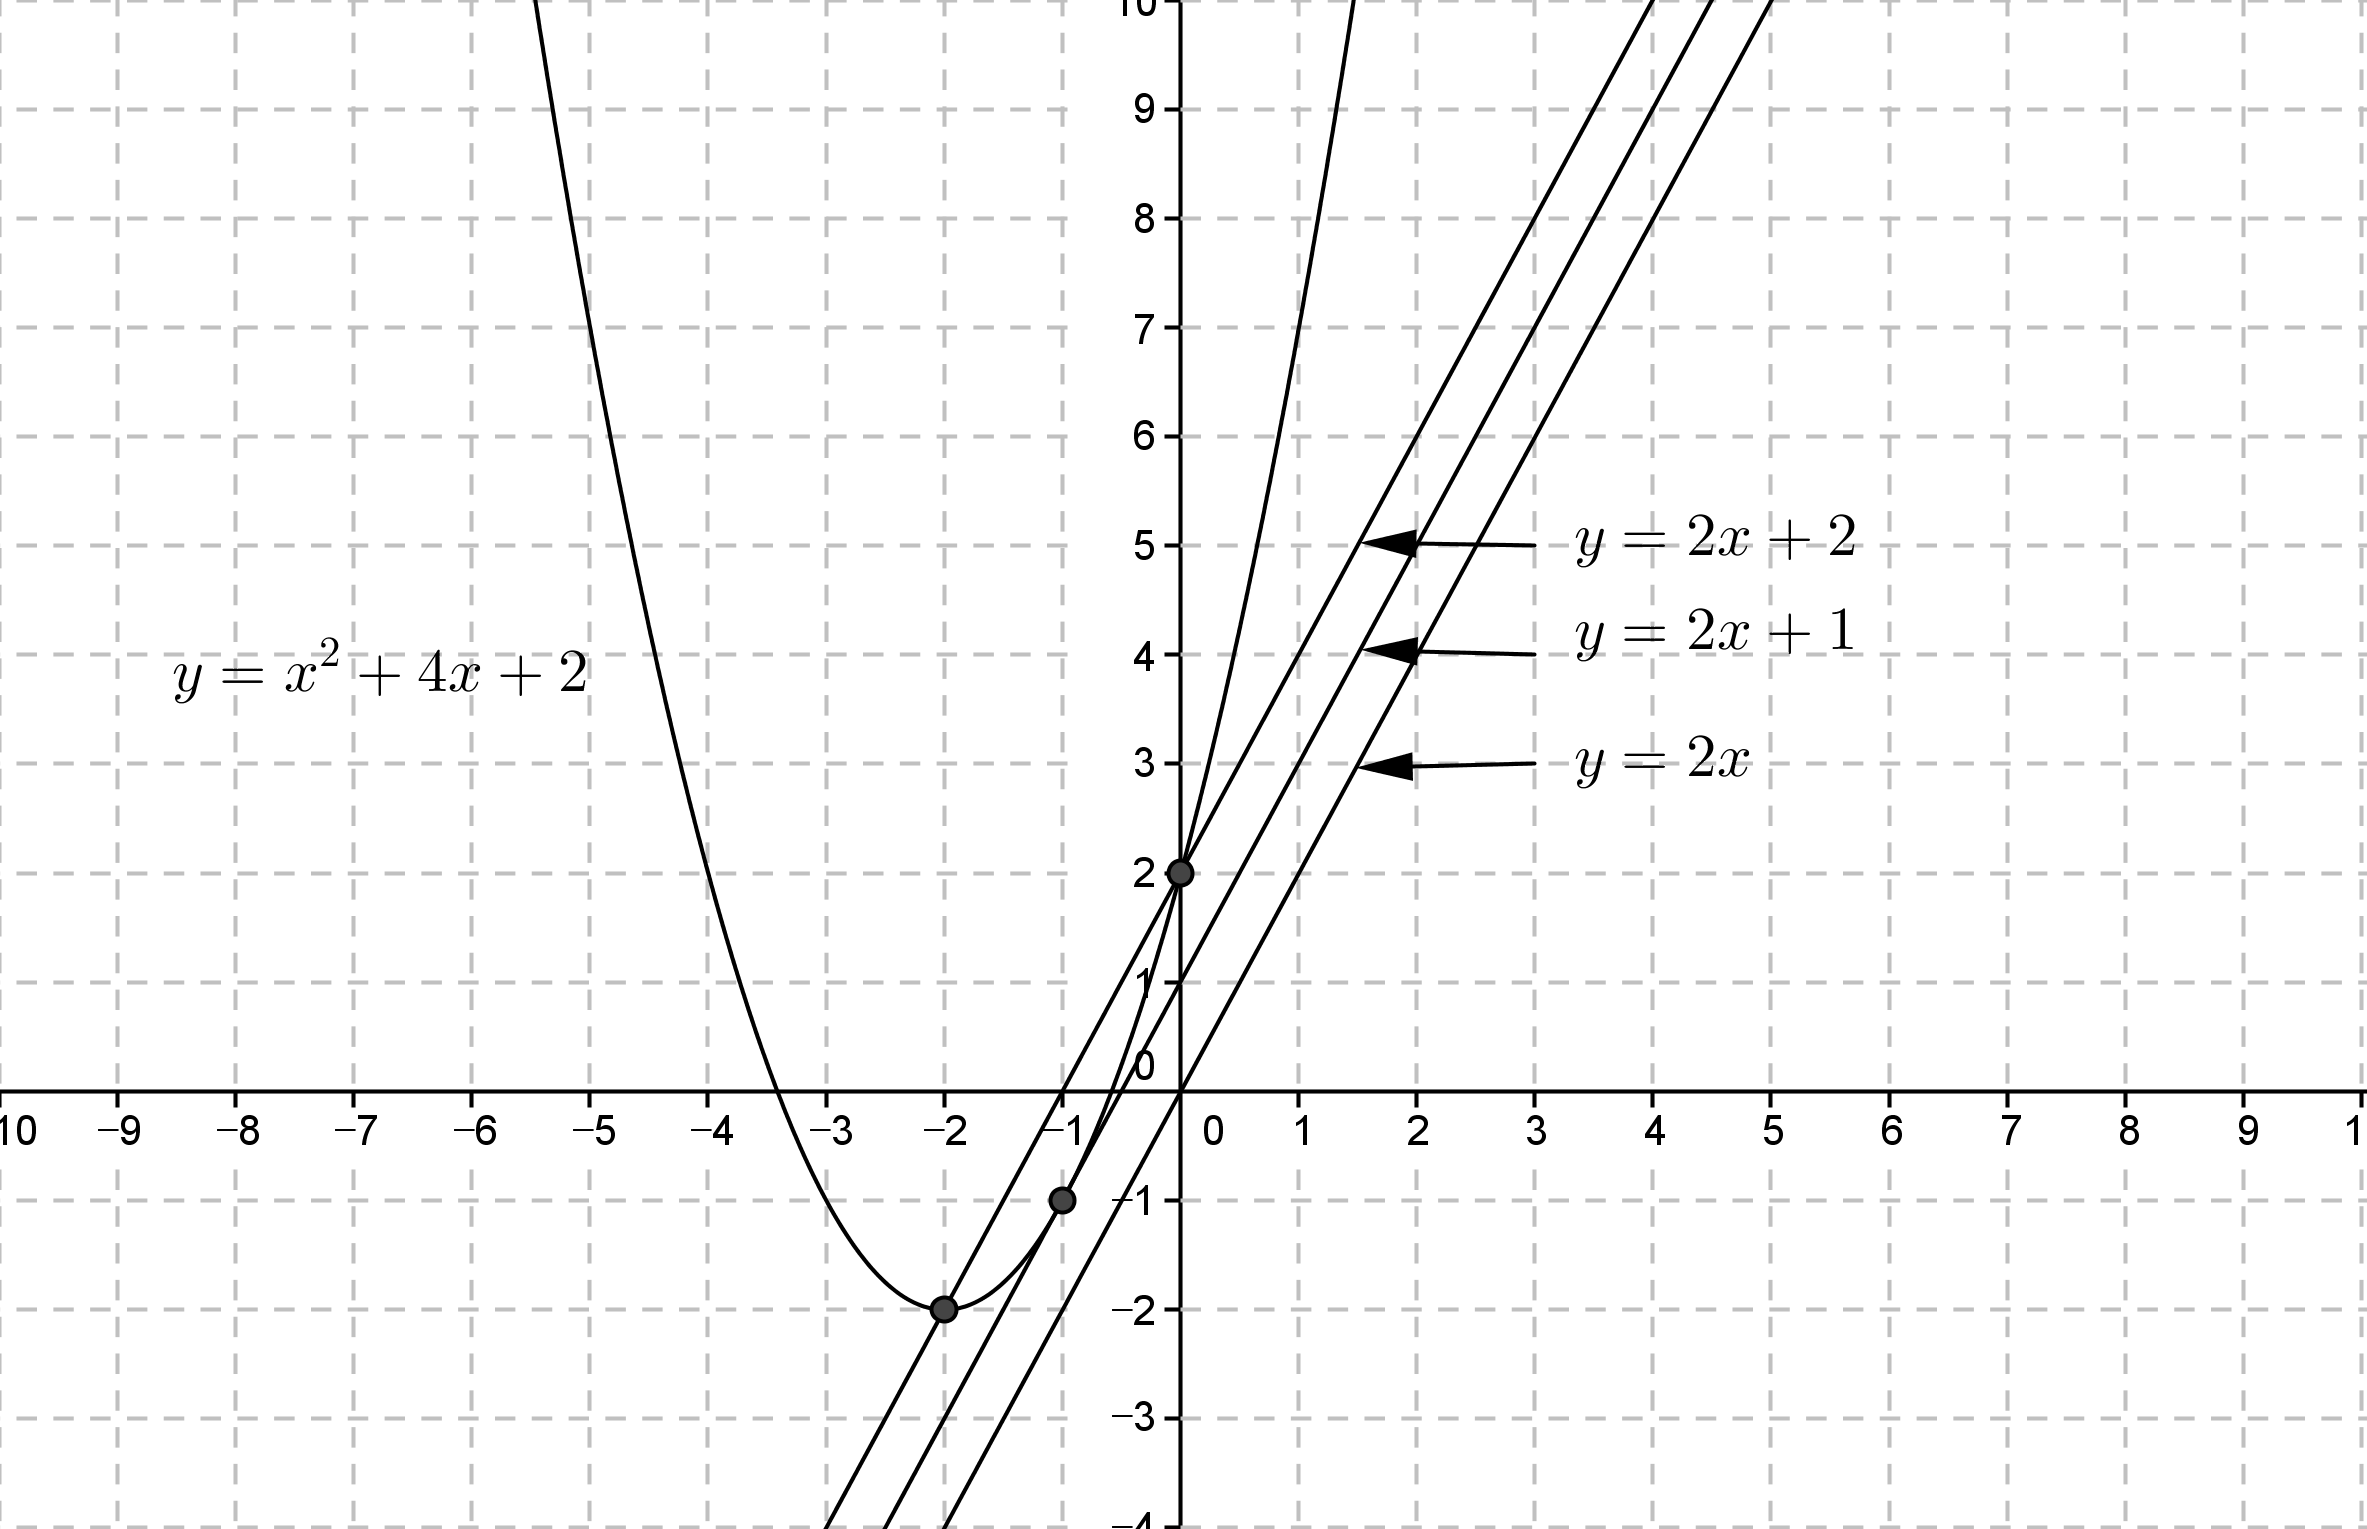
\includegraphics[width=.5\textwidth]{06_01_quad_line}
\end{figure}
이므로 위 결론들이 모두 성립한다는 것을 알 수 있다.

%%
\subsection{이차함수의 최대와 최소}
%
\exam{}
이차함수 \(y=2x^2-4x-1\)은
\begin{align*}
y
&=2x^2-4x-1\\
&=2(x^2-2x)-1\\
\end{align*}
이고 \(-2x=2px\), \(p=-1\), \((x-1)^2=x^2-2x+1\)이므로
\begin{align*}
y
&=2(x^2-2x)-1\\
&=2(x^2-2x+1-1)-1\\
&=2(x^2-2x+1)-2-1\\
&=2(x-1)^2-3
\end{align*}
이다.

따라서
\(y\)는 최솟값 \(-3\)을 가진다.

\begin{figure}[h]
\center
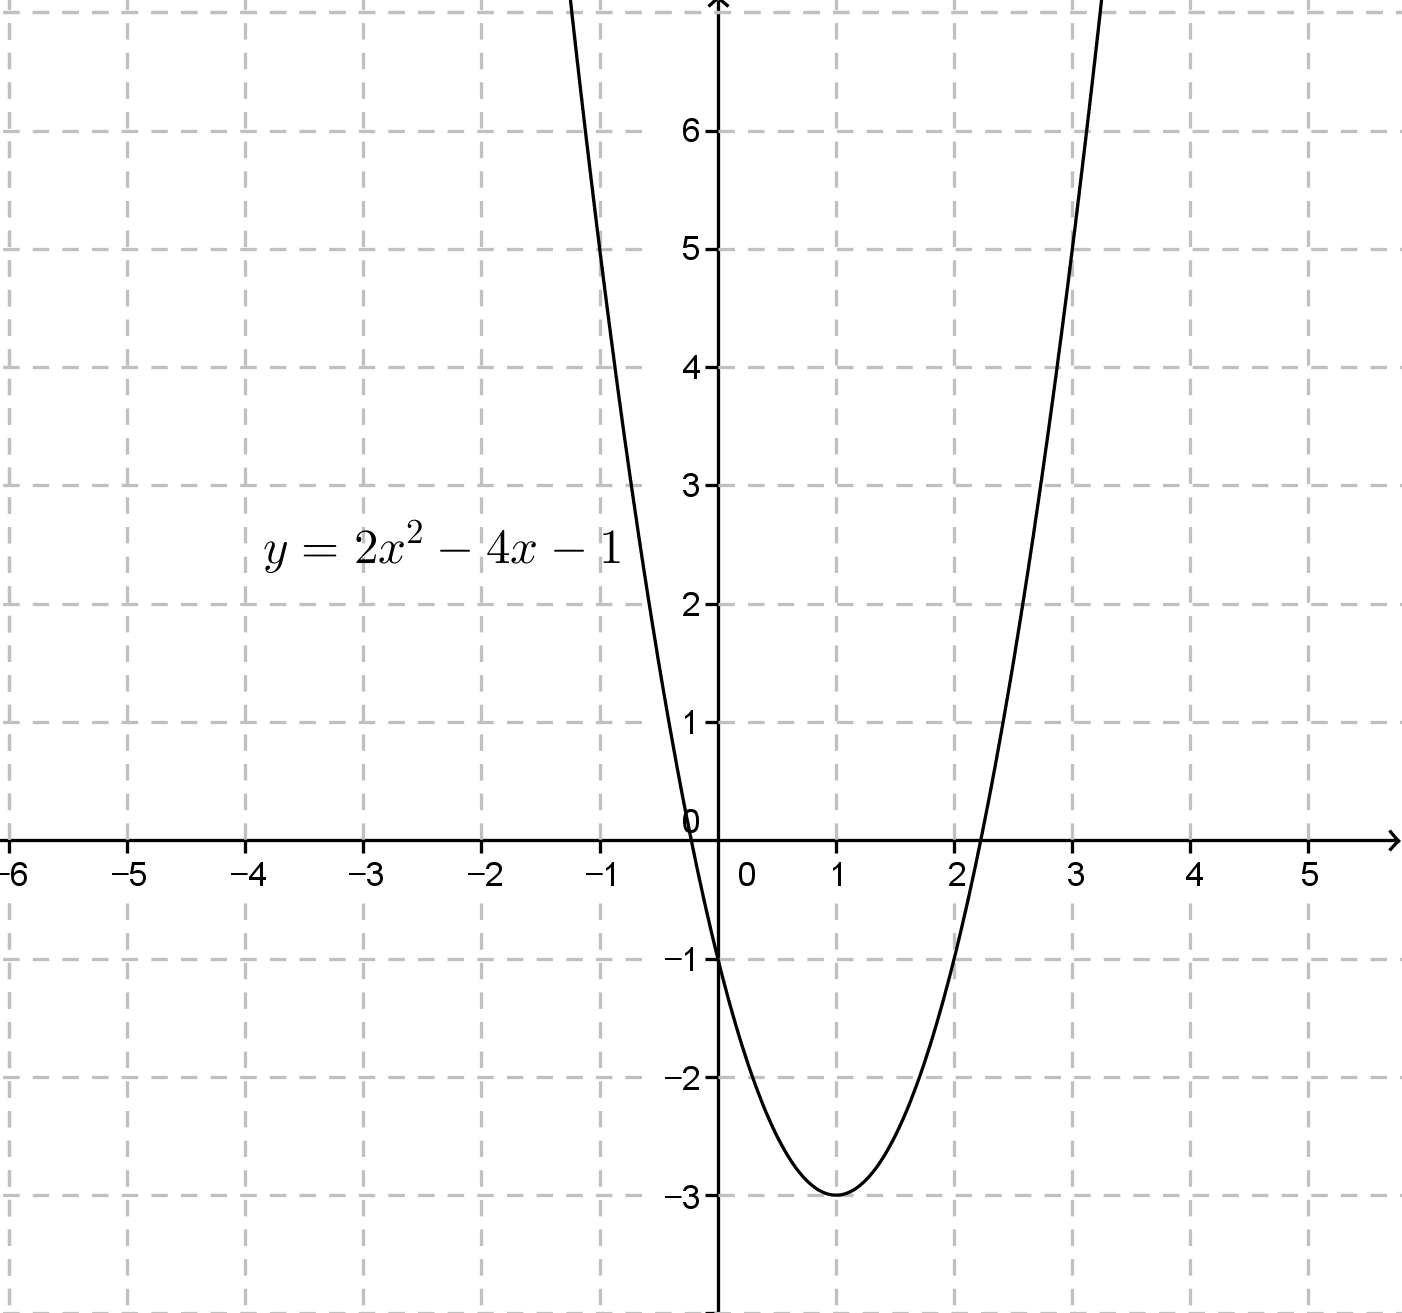
\includegraphics[width=0.5\textwidth]{06_03_maximum}
\end{figure}

이 함수의 최댓값은 없다.

%%%
\section{고차방정식}

\exam{}
고차방정식 \(x^3-3x+2=0\)을 풀어보자.
예시 \ref{fac.x^3-3x+2}에서 \(x^3-3x+2\)가 \((x-1)^2(x+2)\)로 인수분해 될 수 있음을 확인했으므로
\[(x-1)^2(x+2)=0\]
이다.
따라서 \(x-1=0\)이거나 \(x+2=0\)이다.
즉 \(x=1\)이거나 \(x=-2\)이다.

%
\exam{}
고차방정식 \(x^3-3x^2-x+3=0\)을 풀어보자.

\begin{figure}[h]
\center
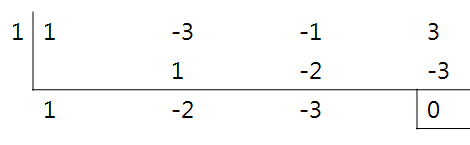
\includegraphics[width=0.5\textwidth]{07_x^3-3x^2-x+3=0}
\end{figure}
에 의해
\begin{align*}
x^3-3x^2-x+3
&=(x-1)(x^2-2x-3)\\
&=(x-1)(x+1)(x-3)=0
\end{align*}
이다.

따라서 \(x=1\), \(x=-1\), \(x=3\)이다.

고차방정식 \(x^3-1=0\)을 풀어보자.
정리 \ref{fac.formula}의 (8)에 의해
\[(x-1)(x^2+x+1)=0\]
이다.
따라서 \(x-1=0\)이거나 \(x^2+x+1=0\)이다. \(x-1=0\)이면 \(x=1\)이고 \(x^2+x+1=0\)이면 근의 공식에 의해 \(x=\frac{-1\pm\sqrt3i}2\)이다.

%%%
\section{연립방정식}

%
\exam{}
연립방정식
\setcounter{equation}{0}
\begin{gather}
x-y+z=1\\
x+2y-z=2\\
-2x+y-3z=-4
\end{gather}
을 풀어보자.

(1)\(+\)(2)를 하면
\[
2x+y=3\tag{4}
\]
이다.
3\(\times\)(1)\(+\)(3)을 하면
\[
x-2y=-1\tag{5}
\]
이다.
2\(\times\)(4)\(+\)(5)를 하면
\[
5x=5
\]
가 되어 \(x=1\)이다.
이것을 다시 (4)에 대입하면 \(y=1\)이다.
또 \(x=1\)과 \(y=1\)을 (1)에 대입하면 \(z=1\)을 얻는다.

따라서 \(x=1\), \(y=1\), \(z=1\)이다.

%
\exam{}
연립방정식
\setcounter{equation}{0}
\begin{gather}
x+y=1\\
x^2+y^2=13
\end{gather}
을 풀어보자.
(1)에서
\[y=1-x\tag{3}\]이다.
이를 (2)에 대입하면
\begin{gather*}
x^2+(1-x)^2=13\\
x^2+(x^2-2x+1)=13\\
2x^2-2x-12=0\\
x^2-x-6=0\\
(x-3)(x+2)=0
\end{gather*}
이므로 \(x=-2\)이거나 \(x=3\)이다.
\(x=-2\)이면 (3)에 의해 \(y=1-(-2)=3\)이고 \(x=3\)이면 \(y=1-3=-2\)이다.

따라서 \(x=-2\), \(y=3\)이거나 \(x=3\), \(y=-2\)이다.
\end{document}